\documentclass[11pt,a4paper]{article}

% Packages
\usepackage[utf8]{inputenc}
\usepackage[T1]{fontenc}
\usepackage{amsmath,amssymb,amsthm}
\usepackage{mathtools}
\usepackage{graphicx}
\usepackage{booktabs}
% Hyperlinks (disable duplicate anchor names)
\usepackage[hypertexnames=false]{hyperref}
% \usepackage{cleveref}  % Not available in basic TeX Live
% \usepackage{algorithm}  % Not needed
% \usepackage{algorithmic}  % Not needed
% \usepackage{natbib}  % Not available in basic TeX Live
\usepackage{geometry}
\usepackage{float}
% \usepackage{subcaption}  % Not available in basic TeX Live
% \usepackage{xcolor}  % Not available in basic TeX Live

% Minimal reference helpers (cleveref not available in basic TeX Live).
% We infer the reference type from the label prefix (e.g., fig:..., thm:..., sec:...).
\makeatletter
\def\Cref@getprefix#1:#2\relax{#1}
\def\Cref@prefix@sec{sec}
\def\Cref@prefix@fig{fig}
\def\Cref@prefix@tab{tab}
\def\Cref@prefix@eq{eq}
\def\Cref@prefix@thm{thm}
\def\Cref@prefix@prop{prop}
\def\Cref@prefix@lem{lem}
\def\Cref@prefix@cor{cor}
\def\Cref@prefix@conj{conj}
\def\Cref@prefix@def{def}
\def\Cref@prefix@rem{rem}
\def\Cref@prefix@ex{ex}

\def\Cref@type@cap#1{%
  \edef\Cref@tmp{#1}%
  \ifx\Cref@tmp\Cref@prefix@sec Section%
  \else\ifx\Cref@tmp\Cref@prefix@fig Figure%
  \else\ifx\Cref@tmp\Cref@prefix@tab Table%
  \else\ifx\Cref@tmp\Cref@prefix@eq Equation%
  \else\ifx\Cref@tmp\Cref@prefix@thm Theorem%
  \else\ifx\Cref@tmp\Cref@prefix@prop Proposition%
  \else\ifx\Cref@tmp\Cref@prefix@lem Lemma%
  \else\ifx\Cref@tmp\Cref@prefix@cor Corollary%
  \else\ifx\Cref@tmp\Cref@prefix@conj Conjecture%
  \else\ifx\Cref@tmp\Cref@prefix@def Definition%
  \else\ifx\Cref@tmp\Cref@prefix@rem Remark%
  \else\ifx\Cref@tmp\Cref@prefix@ex Example%
  \else Ref.%
  \fi\fi\fi\fi\fi\fi\fi\fi\fi\fi\fi\fi
}

\def\Cref@type@low#1{%
  \edef\Cref@tmp{#1}%
  \ifx\Cref@tmp\Cref@prefix@sec section%
  \else\ifx\Cref@tmp\Cref@prefix@fig figure%
  \else\ifx\Cref@tmp\Cref@prefix@tab table%
  \else\ifx\Cref@tmp\Cref@prefix@eq equation%
  \else\ifx\Cref@tmp\Cref@prefix@thm theorem%
  \else\ifx\Cref@tmp\Cref@prefix@prop proposition%
  \else\ifx\Cref@tmp\Cref@prefix@lem lemma%
  \else\ifx\Cref@tmp\Cref@prefix@cor corollary%
  \else\ifx\Cref@tmp\Cref@prefix@conj conjecture%
  \else\ifx\Cref@tmp\Cref@prefix@def definition%
  \else\ifx\Cref@tmp\Cref@prefix@rem remark%
  \else\ifx\Cref@tmp\Cref@prefix@ex example%
  \else ref.%
  \fi\fi\fi\fi\fi\fi\fi\fi\fi\fi\fi\fi
}

\DeclareRobustCommand{\Cref}[1]{%
  \begingroup
  \edef\Cref@label{#1}%
  \edef\Cref@prefix{\expandafter\Cref@getprefix\Cref@label:\relax}%
  \hyperref[#1]{\Cref@type@cap{\Cref@prefix}~\ref*{#1}}%
  \endgroup
}
\DeclareRobustCommand{\cref}[1]{%
  \begingroup
  \edef\Cref@label{#1}%
  \edef\Cref@prefix{\expandafter\Cref@getprefix\Cref@label:\relax}%
  \hyperref[#1]{\Cref@type@low{\Cref@prefix}~\ref*{#1}}%
  \endgroup
}
\makeatother

\geometry{margin=1in}
\setlength{\emergencystretch}{2em} % reduce overfull lines without \sloppy

% Theorem environments
\theoremstyle{plain}
\newtheorem{theorem}{Theorem}[section]
\newtheorem{lemma}[theorem]{Lemma}
\newtheorem{proposition}[theorem]{Proposition}
\newtheorem{corollary}[theorem]{Corollary}
\newtheorem{conjecture}[theorem]{Conjecture}

\theoremstyle{definition}
\newtheorem{definition}[theorem]{Definition}
\newtheorem{example}[theorem]{Example}

\theoremstyle{remark}
\newtheorem{remark}[theorem]{Remark}

% Custom commands
\newcommand{\R}{\mathbb{R}}
\newcommand{\Z}{\mathbb{Z}}
\newcommand{\N}{\mathbb{N}}
\newcommand{\Cov}{\mathrm{Cov}}
\newcommand{\Var}{\mathrm{Var}}

% Stats placeholders (populated by script)
\newcommand{\numMagicThree}{8}
\newcommand{\totalArrangementsThree}{362880}
\newcommand{\magicProbabilityThree}{45,360}
\newcommand{\hullVolumeThree}{18.0000}
\newcommand{\hullAreaThree}{46.2750}
\newcommand{\covXZMagic}{0}
\newcommand{\covYZMagic}{0}
\newcommand{\covXZRandomMean}{0_RANDOM}
\newcommand{\covXZRandomStd}{0_STD}
\newcommand{\perturbPropLarger}{100.0}

\title{\textbf{Magic Gems: A Polyhedral Framework for Magic Squares}\\
\large Connecting Combinatorics, Geometry, and Linear Algebra}

\author{Kyle Elliott Mathewson\\
\textit{Faculty of Science, University of Alberta}\\
\texttt{kyle.mathewson@ualberta.ca}}

\date{\today}

\begin{document}

\maketitle

\begin{abstract}
We introduce \emph{Magic Gems}, a geometric representation of magic squares as three-dimensional polyhedra. 
By mapping an $n \times n$ magic square onto a centered coordinate grid with cell values as vertical displacements, 
we construct a point cloud whose convex hull defines the Magic Gem.
Building on prior work connecting magic squares to physical properties such as moment of inertia,
this construction reveals an explicit statistical structure: 
we show that magic squares have vanishing covariances between position and value.
We develop a covariance energy functional---the sum of squared covariances with row, column, 
and diagonal indicator variables---and establish rigorously for $n=3$ (via exhaustive enumeration) 
that its zeros correspond precisely to magic squares.
Large-scale sampling for $n = 4,5$ (460+ million arrangements) provides strong numerical evidence 
that this characterization extends to larger orders.
Perturbation analysis demonstrates that magic squares are isolated local minima.
The representation is invariant under dihedral symmetry $D_4$, 
yielding canonical geometric objects for equivalence classes.

\medskip
\noindent\textbf{Keywords:} Magic squares, convex polyhedra, covariance, energy landscape, combinatorial geometry
\end{abstract}


\section{Introduction}
\label{sec:introduction}

Magic squares are among the oldest objects of recreational mathematics: the $3\times3$ Lo Shu appears in Chinese sources more than two millennia old, a $4\times4$ square is engraved in D\"urer's \emph{Melencolia~I} (1514), and systematic constructions for every order have been known since the seventeenth century \cite{andrews1960magic,pickover2002zen}.
The modern literature treats them from several directions: enumeration and the geometry of the associated polytopes \cite{stanley1973magic,ehrhart1973magic,ahmed2003polyhedral,beck2006insideout,beck2010enumeration}, spectral and matrix properties \cite{loly2009spectra,nordgren2012properties,nordgren2014spectra,cameron2013signatura}, and, in work of Loly and collaborators, physical invariants such as the moment of inertia and the multipole moments \cite{loly2004invariance,rogers2004inertia,rogers2005multipole}.

\begin{definition}[Magic square]
\label{def:magic_square}
An \emph{arrangement} of order $n$ is a bijection $S=(s_{ij})$ from the cells of the $n\times n$ grid onto $\{1,\dots,n^2\}$.
It is a \emph{magic square} if every row, every column and both main diagonals sum to the magic constant $M(n)=n(n^2+1)/2$, and \emph{semi-magic} if only the rows and columns do.
\end{definition}

This paper studies a three-dimensional representation of an arrangement: place the centred entry $s_{ij}-(n^2+1)/2$ as a height over the centred cell $(j-\frac{n-1}2,\ \frac{n-1}2-i)$ and take the convex hull of the $n^2$ points, the \emph{Magic Gem} of $S$ (\Cref{sec:gem}).
The representation is invariant under the dihedral group $D_4$ of the square, so each essentially different magic square has a single gem (\Cref{prop:symmetry_invariance}); an interactive web application displays the $880$ essentially different order-four squares and renders the gem of a selected one (points, convex hull, vectors from the centre, coordinate axes; rotatable, with orthographic views) at \url{https://kylemath.github.io/MagicGemWebpage/}.
The convex hull itself is the object of Sections~\ref{sec:gem-geometry-880}--\ref{sec:siamese-gems} (the geometry of the $880$ order-four gems and of the Siamese gems); everywhere else the object is the height function $z$.
Once the entries are read as a function on the grid, every line-sum condition ``row $k$ sums to $M(n)$'' becomes ``$z$ is orthogonal to the centred indicator of row $k$'', i.e.\ $\Cov(R_k,Z)=0$ for the empirical covariance over the $n^2$ cells.
A magic square is therefore an arrangement whose height function is orthogonal to a fixed $2n$-dimensional space $W$ of test functions, and the natural \emph{energy} $\Efull(S)=\sum_L\Cov(\mathbf 1_L,Z)^2$ over the $2n+2$ lines vanishes exactly on magic squares (\Cref{lem:zero_set}).
We are explicit that this is a reformulation of the definition and not a theorem about magic squares (\Cref{rem:tautology}); its value is that it suggests questions whose answers are not visible in the line-sum formulation, and the paper is organised around those answers.

\paragraph{Contributions.}
\begin{enumerate}\setlength\itemsep{1pt}
\item \emph{The moment hierarchy} (\Cref{prop:hierarchy}, \Cref{thm:perm_threshold}). Replacing the line indicators by the polynomial test functions $x^m,y^m$ gives, for each degree $k$, the conditions $\Cov(X^m,Z)=\Cov(Y^m,Z)=0$ for $m\le k$. For real-valued height functions these are equivalent to equal row and column sums if and only if $k\ge n-1$; this is the invertibility of a Vandermonde matrix and we state it as a proposition. The result of the section is \Cref{thm:perm_threshold}: for permutations of $1,\dots,n^2$, integrality and the bound on line sums force the threshold $k^*(n)$ down to at most $n-2$ for every $n\ge14$, whereas $k^*(n)=n-1$ for $3\le n\le13$ (computer-verified witnesses, \Cref{rem:kstar_search}). The ``low-mode'' energy $\Elow$ of earlier versions of this paper is the degree-one truncation. Loly's invariance of the moment of inertia \cite{loly2004invariance}, which Loly derived from the row and column sums alone and so stated for semi-magic squares, is the single condition $\Cov(Z,X^2+Y^2)=0$: implied by the degree-two conditions, but much weaker than them (\Cref{cor:loly}). The same identity gives the null distribution of the moment of inertia of a random arrangement (\Cref{cor:loly_null}).
\item \emph{Exact statistics of a random arrangement} (\Cref{prop:random_energy_moments}). $\E[\Elow]=(n^2+1)(n^4-n^2+12n-12)/(72n^2)$ and $\E[\Efull]=(n^4-1)/(6n^2)$, with exact variances; $\Elow/\E[\Elow]\to\mathrm{Exp}(1)$ by Hoeffding's combinatorial central limit theorem. Monte Carlo with $10^8$ samples per order agrees for $n\le 8$ to within $5\times10^{-4}$ relative error.
\item \emph{The single-swap formula} (\Cref{thm:swap}). Exchanging two entries of a magic square that differ by $d$ raises $\Efull$ by exactly $d^2m/n^4$, where $m\in\{2,\dots,6\}$ counts the lines separating the two cells; every magic square is a strict local minimum, with minimum gap between $2/n^4$ and $6/n^4$.
\item \emph{The low-mode class for $n=4$} (\Cref{prop:L4}). Exactly $14{,}639{,}440$ of the $16!$ arrangements satisfy $\Elow=0$, $7{,}040$ of them magic; the count is a meet-in-the-middle enumeration and agrees with a Gaussian local-limit estimate to within $20\%$.
\item \emph{Geometry of the $880$ order-four gems} (\Cref{sec:gem-geometry-880}). $8$ to $16$ hull vertices, $39$ $f$-vectors, $352$ combinatorial types and $616$ congruence classes, which are exactly the orbits of the complement map $S\mapsto17-S$; no two gems have the same hull-vertex set. The Siamese squares of every odd order $n\ge5$ have gems with exactly twelve vertices (\Cref{prop:siamese-12}, computer-assisted proof).
\end{enumerate}

\paragraph{What is and is not new.}
The polyhedral geometry of magic squares is classical: nonnegative integer matrices with all line sums equal to $t$ are the lattice points of the $t$-th dilate of the Birkhoff polytope and their number is a polynomial in $t$ \cite{stanley1973magic,ehrhart1973magic}; the count of magic squares with distinct entries is an Ehrhart quasi-polynomial of an inside-out polytope \cite{beck2006insideout,beck2010enumeration}; the cones of magic squares and cubes have Hilbert-basis descriptions \cite{ahmed2003polyhedral}.
The Magic Gem is a different object: not the polytope whose lattice points are the squares, but a polyhedron attached to one square.
The orthogonality reading of the constraints is elementary and implicit in Loly's work, and the hierarchy itself is elementary: that the axial moments $\sum_{ij}s_{ij}x_j^m$ of a semi-magic object vanish for every $m$ is, in physical language, the vanishing of its multipole moments, as Rogers and Loly observed for the dipole and quadrupole moments of a magic cube \cite{rogers2005multipole}.
What is new is the converse threshold and its permutation refinement (\Cref{thm:perm_threshold}), the exact random-arrangement moments, the swap formula, the exact low-mode count, and the exact geometry of the $880$ gems.
We make no claim that the energy reformulation by itself is a result.

\paragraph{Corrections relative to version 4 (arXiv:2512.09170v4).}
\begin{itemize}\setlength\itemsep{0pt}
\item[(a)] The complete energy used there omitted one row and one column and was not $D_4$-invariant; all statistics now use the symmetric sum \eqref{eq:Efull}.
\item[(b)] The sampled statistics (means $4.44$, $12.04$, $26.00$), the ``landscape entropy'' and the quadratic fits had the diagonal terms weighted by $n^2$; withdrawn, replaced by \Cref{prop:random_energy_moments}.
\item[(c)] The ``trimodal'' swap gaps and the ``$1/n^2$'' minimum-gap scaling were artifacts: gaps are $d^2m/n^4$ and $\Delta_{\min}=\Theta(n^{-4})$ with constants $2$, $6$ (\Cref{cor:local_min}).
\item[(d)] The $24$ local minima of $\Efull$ for $n=3$ referred to the asymmetric energy; the symmetric one has $16$ (\Cref{sec:n3_exhaustive}).
\item[(e)] ``$\Elow=0$ characterises magic (or semi-magic) squares'' is withdrawn (\Cref{rem:four_term_insufficient}, \Cref{prop:L4}); $P(\Elow=0)$ for $n=4$ is $7.0\times10^{-7}$, not ``below $10^{-8}$'', and the statement that $6\times10^7$ samples for $n=4$ and $4\times10^8$ for $n=5$ contained no zero is unsupported by the archived data, which hold $10^5$ samples per order; the cause cannot be reconstructed from the repository (\Cref{sec:lowmode_n4}).
\item[(f)] Table~2 of v4 (``typical'' $16$ hull vertices for $n=5$, volume $95.0$ for $n=4$) is replaced by exact values for named squares (\Cref{sec:gem-geometry-880}); the hardware statement is corrected (\Cref{sec:appendix}).
\end{itemize}

\Cref{sec:background} collects the facts we use; \Cref{sec:gem} defines the gem; \Cref{sec:theory} contains the projection lemma, the hierarchy and the swap formula; \Cref{sec:results} the computations; \Cref{sec:discussion} what the viewpoint does and does not buy, local search, and open questions; the appendices the methods, the variance closed forms, the witnesses and the remaining steps of the Siamese proof.


\section{Background}
\label{sec:background}

\subsection{Enumeration and symmetry}

There are $8$ magic squares of order $3$, all images of the Lo Shu under the dihedral group $D_4$ of the square (four rotations, four reflections); there are $7{,}040$ of order $4$, forming $880$ $D_4$-orbits first listed by Fr\'enicle de Bessy (published posthumously in 1693) and verified many times since \cite{beck2010enumeration}; and $275{,}305{,}224$ of order $5$, counted by Schroeppel in 1973 and reported by Gardner \cite{gardner1976}, i.e.\ $34{,}413{,}153$ orbits.
For $n\ge6$ only statistical estimates are known; see Trump's compilation \cite{trump2012enumeration}.
Since $D_4$ maps lines to lines and preserves the entry set, it maps magic squares to magic squares, and two squares in the same orbit are called \emph{essentially different} from squares in other orbits.
The $880$ order-four squares were further sorted by Dudeney into twelve groups according to the pattern of complementary pairs $(a,17-a)$ \cite{dudeney1917amusements}; we use these groups only as a classical reference partition in \Cref{sec:gem-geometry-880}.
Classical constructions (Siamese for odd $n$, diagonal-complement for $n\equiv0\pmod 4$, LUX or Strachey for $n\equiv2\pmod4$) show that magic squares exist for all $n\ge3$ \cite{andrews1960magic}; we use the Siamese squares as a family on which hull computations can be pushed to large $n$.

\subsection{Covariance and the inertia tensor}
\label{sec:bg_inertia}

For a finite point set $\mathbf p_1,\dots,\mathbf p_N\in\R^3$ with mean $\bar{\mathbf p}$, the covariance matrix is $\Sigma_{jk}=\frac1N\sum_i(p_{i,j}-\bar p_j)(p_{i,k}-\bar p_k)$.
With unit masses at the points, the inertia tensor about the centre of mass is
\begin{equation}
I_{jk}=\sum_i\bigl(\|\mathbf p_i-\bar{\mathbf p}\|^2\delta_{jk}-(p_{i,j}-\bar p_j)(p_{i,k}-\bar p_k)\bigr)
=N\bigl(\delta_{jk}\operatorname{tr}\Sigma-\Sigma_{jk}\bigr),
\label{eq:inertia_cov}
\end{equation}
where $\delta_{jk}$ is the Kronecker delta \cite{goldstein2002classical}.
Thus the off-diagonal entries of $I$ are $-N$ times the covariances and the diagonal entries are $N$ times the sum of the two other variances.
Loly's planar moment of inertia \cite{loly2004invariance} is a different object: it places the \emph{value} $s_{ij}$ as a mass at the planar point $(x_{ij},y_{ij})$ and computes $\sum s_{ij}(x_{ij}^2+y_{ij}^2)$.
The two are nevertheless related through the gem's point set: Loly's quantity is an affine function of the single degree-two cross-moment $\Cov(Z,X^2+Y^2)$ of that point set (\Cref{cor:loly}), and this is the only ingredient of the three-dimensional covariance $\Sigma$ that it uses.

\subsection{Two tools from permutation statistics}
\label{sec:bg_perm}

Let $\pi$ be a uniformly random permutation of $\{1,\dots,N\}$ and $a,b\in\R^N$ fixed vectors.
The quantity $T_a=\sum_i a_i b_{\pi(i)}$ is a \emph{linear permutation statistic}.
Its mean is $N\bar a\bar b$ and, for two such statistics with the same $b$ (Wald--Wolfowitz \cite{waldwolfowitz1944}, polarised),
\begin{equation}
\Cov(T_a,T_{a'})=\frac{1}{N-1}\sum_i(a_i-\bar a)(a'_i-\bar a')\sum_j(b_j-\bar b)^2 .
\label{eq:ww_identity}
\end{equation}
Hoeffding's combinatorial central limit theorem \cite[Thm.~3]{hoeffding1951} gives asymptotic normality of $\sum_i c_N(i,\pi(i))$ when, for every integer $r\ge3$, $N^{-1}\sum_{i,j}|d_N(i,j)|^r$ is $O\bigl((N^{-1}\sum_{i,j}d_N(i,j)^2)^{r/2}\bigr)$, $d_N$ being the doubly centred array; for product arrays $c_N(i,j)=a_ib_j$ the condition reduces to a bound on the standardised absolute moments of $a$ and $b$.
In \Cref{sec:random_energy} the energies of a random arrangement are quadratic forms in such statistics; \eqref{eq:ww_identity} gives their means exactly, and the distribution of a quadratic form in Gaussian variables is computed by Imhof's inversion formula \cite{imhof1961}.

\subsection{Polytopes of magic squares}
\label{sec:bg_polytopes}

The polytope literature on magic squares concerns a different polytope from the one studied here.
An $n\times n$ nonnegative integer matrix with all row and column sums equal to $t$ is a lattice point of the $t$-th dilate of the Birkhoff polytope of doubly stochastic matrices, and their number is a polynomial in $t$ of degree $(n-1)^2$ \cite{stanley1973magic,ehrhart1973magic,ziegler1995lectures}; adding the diagonal conditions and distinct entries leads to the inside-out polytopes of Beck and Zaslavsky \cite{beck2006insideout}, which gave the first enumeration of $4\times4$ magic squares of arbitrary magic sum \cite{beck2010enumeration}; the cones of magic squares and cubes have Hilbert-basis descriptions \cite{ahmed2003polyhedral}; and contingency tables with fixed margins are the same lattice points studied as a sample space \cite{diaconis1995rectangular}.
In all of these the magic squares are the \emph{points} of a polytope, whereas the Magic Gem attaches a polyhedron to a \emph{single} square; the two constructions share nothing beyond the word.
Spectral and matrix properties of a magic square \cite{loly2009spectra,nordgren2012properties,nordgren2014spectra}, the singular-value signatures and entropies of Cameron, Rogers and Loly \cite{cameron2013signatura}, and Loly's physical invariants---the moment of inertia \cite{loly2004invariance}, the inertia tensor and the multipole moments of a magic cube \cite{rogers2004inertia,rogers2005multipole}, and the study of Franklin squares \cite{loly2007franklin}---are closer to our viewpoint: they, too, attach a quantity to one square and ask what it reveals.


\section{Methodology: The Magic Gem Framework}
\label{sec:methodology}

We now develop the Magic Gem framework, beginning with the construction of three-dimensional point clouds 
from magic squares and culminating in our main theoretical result connecting magic squares to zero-covariance configurations.

\subsection{From Magic Square to Point Cloud}

Let $S = (s_{ij})$ be an $n \times n$ magic square with entries $s_{ij} \in \{1, 2, \ldots, n^2\}$.
We construct a point cloud $P \subset \R^3$ by assigning three-dimensional coordinates to each cell of the grid.

\begin{definition}[Magic Gem Coordinates]
\label{def:gem_coords}
For each cell $(i, j)$ with $i, j \in \{0, 1, \ldots, n-1\}$, define the point
\begin{equation}
\mathbf{p}_{ij} = \left( x_{ij}, y_{ij}, z_{ij} \right),
\end{equation}
where the coordinates are given by
\begin{align}
x_{ij} &= j - \frac{n-1}{2}, \label{eq:x_coord} \\
y_{ij} &= \frac{n-1}{2} - i, \label{eq:y_coord} \\
z_{ij} &= s_{ij} - \frac{n^2 + 1}{2}. \label{eq:z_coord}
\end{align}
\end{definition}

The horizontal coordinates $x$ and $y$ place the grid centered at the origin,
with the $x$-axis aligned with columns and the $y$-axis aligned with rows (inverted so that the top row has positive $y$).
For a $3 \times 3$ grid, the nine positions have $x$- and $y$-coordinates in $\{-1, 0, 1\}$;
for a $5 \times 5$ grid, they lie in $\{-2, -1, 0, 1, 2\}$.

The vertical coordinate $z$ encodes the cell's value, shifted so that the mean value $(n^2 + 1)/2$ maps to zero.
This centering ensures that the point cloud has zero mean in all three coordinates,
a property that will prove essential for the covariance analysis.

\begin{example}[Lo Shu Square]
For the Lo Shu square
\[
S = \begin{pmatrix}
2 & 7 & 6 \\
9 & 5 & 1 \\
4 & 3 & 8
\end{pmatrix},
\]
with $n = 3$ and center value $5$, the nine points are
\begin{align*}
\mathbf{p}_{00} &= (-1, 1, -3), & \mathbf{p}_{01} &= (0, 1, 2), & \mathbf{p}_{02} &= (1, 1, 1), \\
\mathbf{p}_{10} &= (-1, 0, 4), & \mathbf{p}_{11} &= (0, 0, 0), & \mathbf{p}_{12} &= (1, 0, -4), \\
\mathbf{p}_{20} &= (-1, -1, -1), & \mathbf{p}_{21} &= (0, -1, -2), & \mathbf{p}_{22} &= (1, -1, 3).
\end{align*}
Note that the center cell, containing the value 5, maps to the origin.
\end{example}

\Cref{fig:construction} illustrates the four-step construction process, 
progressing from the magic square through the centered grid to the final three-dimensional representation,
along with all eight $D_4$ symmetry variants of the Lo Shu square.

\begin{figure}[H]
    \centering
    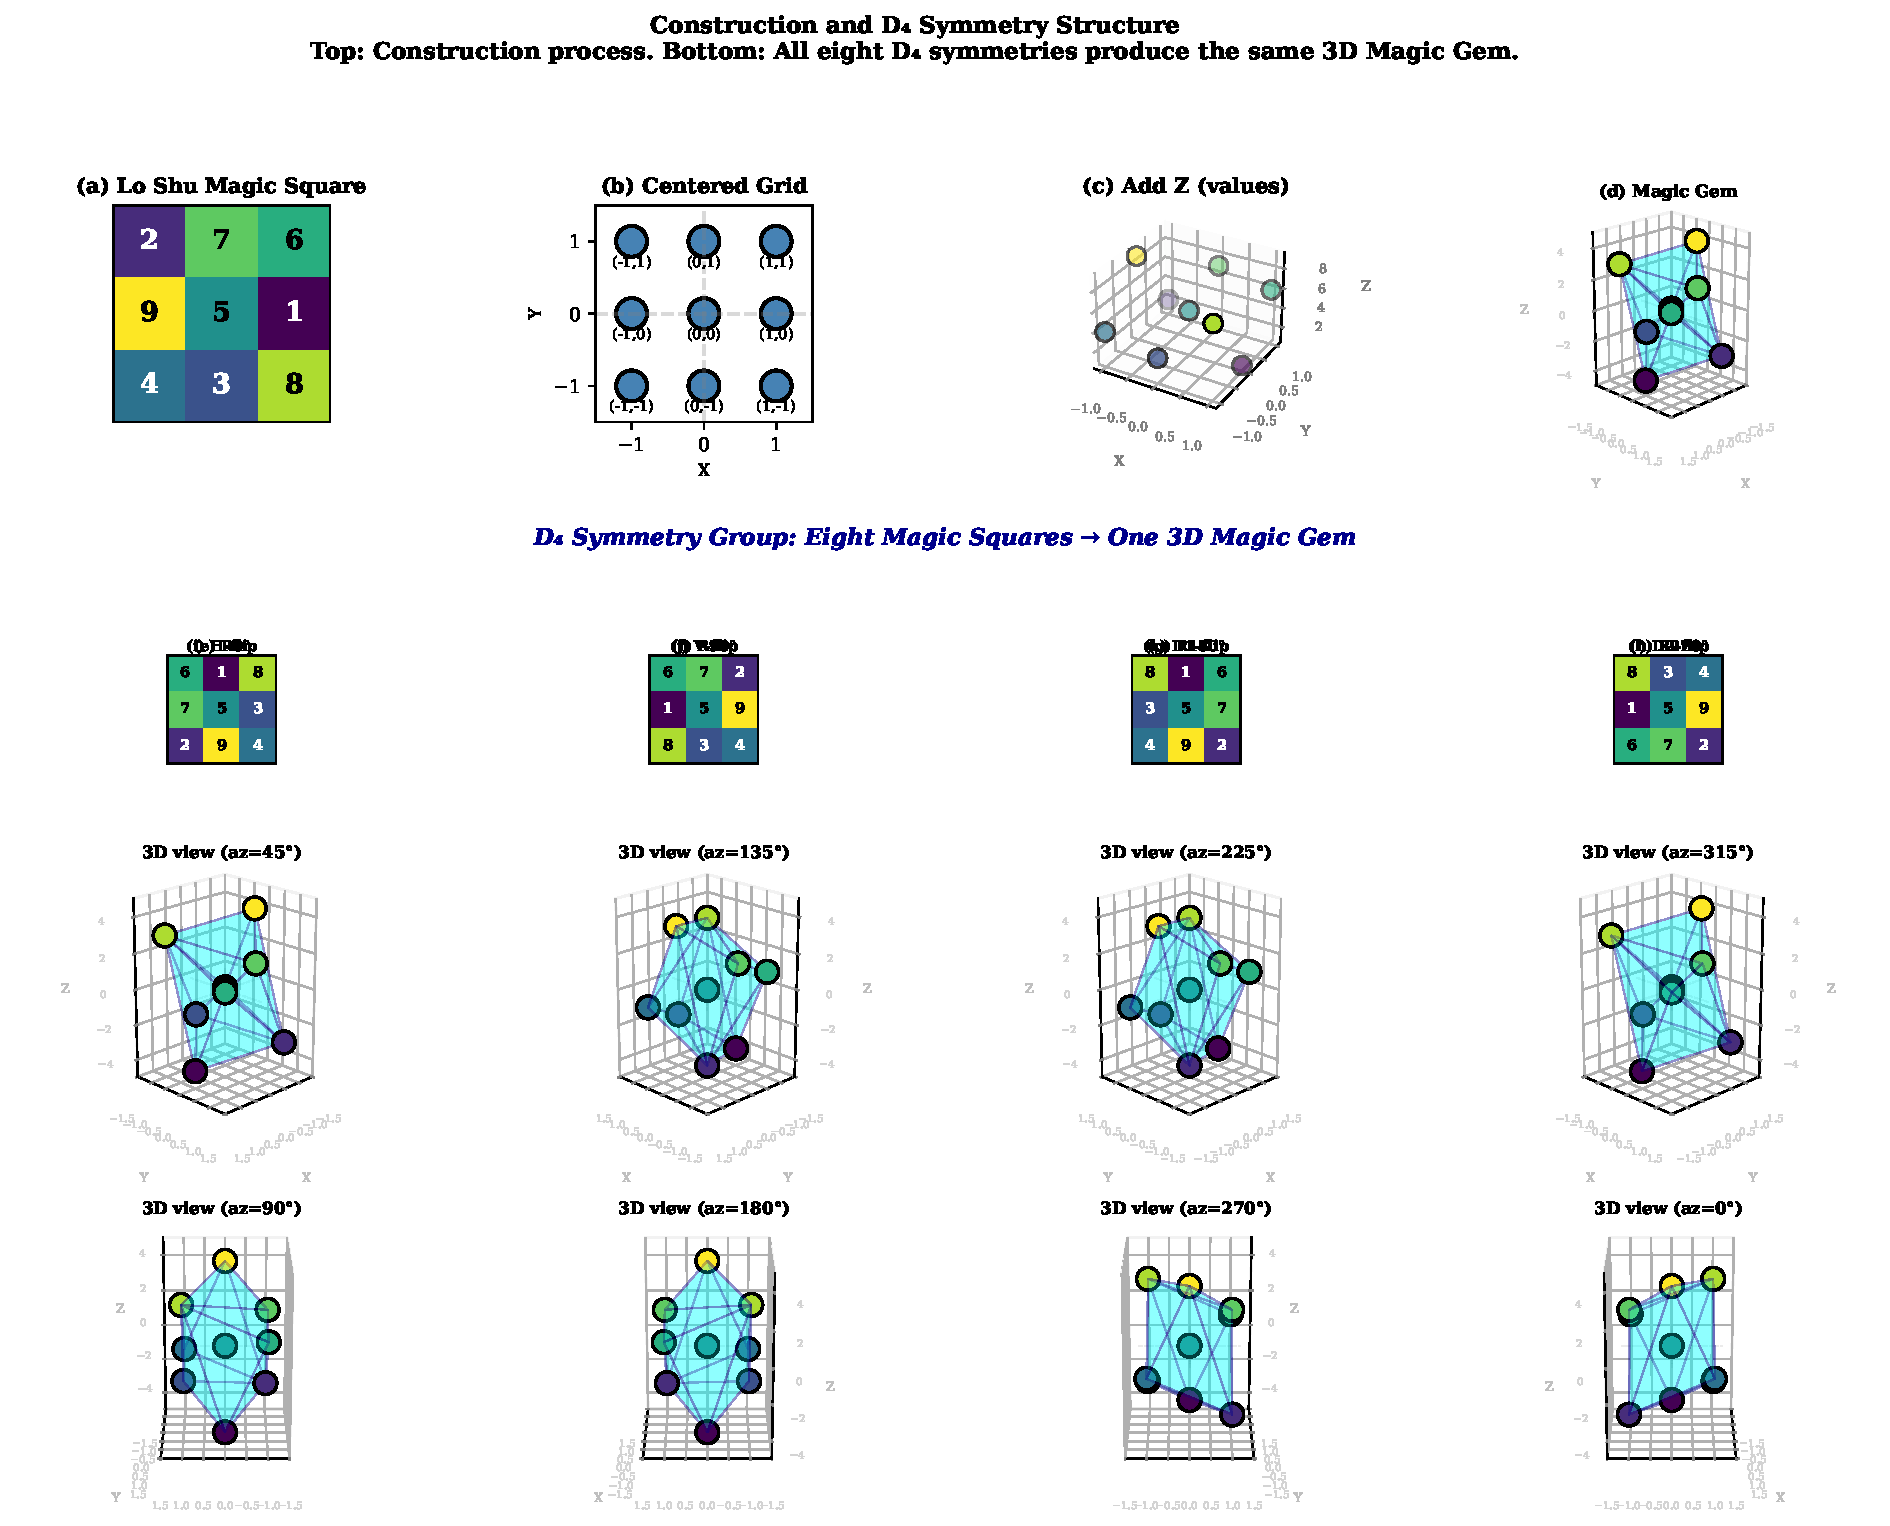
\includegraphics[width=\textwidth]{figures/fig02_combined_construction_symmetries.pdf}
    \caption{\textbf{Construction process and $D_4$ symmetry structure.}
    \emph{Top row (a--d):} Construction of a Magic Gem from the Lo Shu square.
    (a) The Lo Shu magic square---the unique (up to symmetry) $3 \times 3$ magic square, 
    with each row, column, and diagonal summing to $M(3) = 15$.
    (b) Placement on a centered coordinate grid with origin at center.
    (c) Assignment of $z$-values from cell entries.
    (d) Centered Magic Gem point cloud with convex hull.
    \emph{Bottom section (e--l):} The eight $D_4$ symmetries of the $3 \times 3$ magic square.
    Each panel shows a compact 2D magic square (top) paired with its corresponding 3D Magic Gem (bottom, large and prominent).
    The gems are shown from different viewing angles to emphasize their three-dimensional structure.
    Despite their distinct numerical arrangements, all eight $D_4$ variants yield the same 3D Magic Gem polyhedron,
    demonstrating the geometric invariance of the Magic Gem representation under the symmetry group.}
    \label{fig:construction}
\end{figure}

\subsection{The Magic Gem Polyhedron}

With the point cloud defined, we construct the Magic Gem as its convex hull \cite{barvinok2002course}.

\begin{definition}[Magic Gem]
The \emph{Magic Gem} associated with a magic square $S$ is the convex hull of the corresponding point cloud:
\[
\mathcal{G}(S) = \text{conv}\left( \{ \mathbf{p}_{ij} : 0 \leq i, j < n \} \right).
\]
\end{definition}

A fundamental property of this construction is its invariance under the symmetry operations of the magic square.

\begin{proposition}[Symmetry Invariance]
\label{prop:symmetry_invariance}
If $S'$ is obtained from $S$ by a symmetry operation $g \in D_4$, then $\mathcal{G}(S) = \mathcal{G}(S')$.
\end{proposition}

\begin{proof}
Each element $g \in D_4$ acts on the grid as an orthogonal transformation of the $(x, y)$ plane,
which extends naturally to an isometry of $\R^3$ that fixes the $z$-axis direction.
Under this action, the $z$-coordinates are permuted according to the relabeling of cells,
but the set of $z$-values remains unchanged.
Since convex hulls are invariant under isometries and depend only on the set of points (not their labeling),
we have $\mathcal{G}(S) = \mathcal{G}(S')$.
\end{proof}

This invariance means that all eight $D_4$ variants of a magic square produce the same Magic Gem.
For $n = 3$, this implies that the single essentially different magic square yields a unique Magic Gem,
while for larger orders, each equivalence class corresponds to a distinct geometric object.

The construction figure (\Cref{fig:construction}, bottom rows) displays all eight symmetry variants of the $3 \times 3$ magic square,
illustrating how these numerically distinct arrangements share a common geometric representation.

\subsection{The Vector Representation}
\label{sec:vector_rep}

The centering of our coordinate system invites an interpretation of each point as a vector from the origin.
Since the origin coincides with the centroid of the point cloud (as we shall verify),
this vector representation captures the deviation of each cell from the ``balanced'' center.

\begin{definition}[Magic Gem Vectors]
The \emph{vector representation} of a Magic Gem is the collection
\[
\mathcal{V}(S) = \left\{ \mathbf{v}_{ij} = \mathbf{p}_{ij} : 0 \leq i, j < n \right\},
\]
where each point is interpreted as a vector emanating from the origin.
\end{definition}

This interpretation connects the Magic Gem to the classical physics of rigid bodies:
if unit masses are placed at each vertex, the resulting configuration has its center of mass at the origin,
and the vectors $\mathbf{v}_{ij}$ describe the displacement of each mass from this center.

\subsubsection{Vectors and Covariance}

The vector representation provides a geometric interpretation of the zero-covariance condition.
Consider the weighted sum of vectors where each vector is weighted by its $x$-coordinate:
\[
\sum_{i,j} x_{ij} \mathbf{v}_{ij} = \sum_{i,j} x_{ij} (x_{ij}, y_{ij}, z_{ij}).
\]
The $z$-component of this weighted sum is precisely $n^2 \cdot \Cov(X, Z)$.
Thus, zero covariance is equivalent to the statement that vectors, 
when weighted by their horizontal positions, have no net vertical tendency.

More explicitly, define the \emph{position-weighted vector sums}:
\begin{align}
\mathbf{W}_x &= \sum_{i,j} x_{ij} \mathbf{v}_{ij}, \label{eq:weighted_x} \\
\mathbf{W}_y &= \sum_{i,j} y_{ij} \mathbf{v}_{ij}. \label{eq:weighted_y}
\end{align}
Then $\Cov(X, Z) = 0$ if and only if $(\mathbf{W}_x)_z = 0$, 
and $\Cov(Y, Z) = 0$ if and only if $(\mathbf{W}_y)_z = 0$.

This formulation reveals that magic squares achieve a form of \emph{directional balance}:
the $z$-values are distributed so that neither horizontal direction 
exhibits any systematic correlation with value magnitude.
The vectors in Figure panels showing the vector representation 
visually manifest this balance---vectors pointing in each horizontal direction 
have $z$-components that ``cancel out'' when weighted by position.

\subsection{The Covariance Structure of Magic Squares}
\label{sec:zero_cov_theorem}

We now establish our main theoretical results, revealing a deep connection 
between the algebraic definition of magic squares and the statistical structure of Magic Gems.

\subsubsection{Forward Direction: Magic Implies Zero Covariance}

The following result holds for all $n \geq 3$ and admits a clean algebraic proof.

\begin{proposition}[Magic Implies Zero Covariance]
\label{prop:magic_implies_zero_cov}
Let $S$ be an $n \times n$ magic square, and let $P = \{\mathbf{p}_{ij}\}$ be the corresponding point cloud. 
Then $\Cov(X, Z) = \Cov(Y, Z) = 0$.
\end{proposition}

\begin{proof}
We first verify that the means of all three coordinates vanish.
For the $x$-coordinate,
\[
\bar{X} = \frac{1}{n^2} \sum_{i,j} x_{ij} = \frac{1}{n^2} \sum_{i,j} \left( j - \frac{n-1}{2} \right) 
= \frac{n}{n^2} \sum_{j=0}^{n-1} \left( j - \frac{n-1}{2} \right) = 0,
\]
since $\sum_{j=0}^{n-1} j = n(n-1)/2$. An analogous argument shows $\bar{Y} = 0$, and 
\[
\bar{Z} = \frac{1}{n^2} \sum_{i,j} \left( s_{ij} - \frac{n^2+1}{2} \right) = 0
\]
since the entries sum to $n^2(n^2+1)/2$.

With zero means, $\Cov(X, Z) = \frac{1}{n^2} \sum_{i,j} x_{ij} z_{ij}$.
Define $C_j = \sum_{i=0}^{n-1} s_{ij}$ as the sum of column $j$. Then:
\[
\Cov(X, Z) = \frac{1}{n^2} \sum_{j=0}^{n-1} \left( j - \frac{n-1}{2} \right) C_j.
\]
For a magic square, all column sums equal $M(n)$, so
\[
\Cov(X, Z) = \frac{M(n)}{n^2} \sum_{j=0}^{n-1} \left( j - \frac{n-1}{2} \right) = 0.
\]
The argument for $\Cov(Y, Z) = 0$ via row sums is analogous.
\end{proof}

\begin{corollary}
For any magic square, the covariance matrix of the Magic Gem coordinates has the block-diagonal form
\[
\Sigma = \begin{pmatrix}
\Var(X) & \Cov(X,Y) & 0 \\
\Cov(X,Y) & \Var(Y) & 0 \\
0 & 0 & \Var(Z)
\end{pmatrix}.
\]
In particular, the $z$-coordinate is uncorrelated with both horizontal coordinates.
\end{corollary}

\subsubsection{On the Insufficiency of Aggregate Covariances}
\label{sec:insufficiency}

It is natural to ask whether the conditions $\Cov(X, Z) = \Cov(Y, Z) = 0$ alone 
suffice to characterize magic squares, or at least semi-magic squares 
(those with equal row and column sums but possibly failing the diagonal conditions).
Perhaps surprisingly, the answer is \emph{no}---and understanding why reveals 
a crucial distinction that motivates our energy functional approach.

\begin{remark}[Why $\Cov(X,Z)=0$ Is Not Enough]
\label{rem:first_moment}
The condition $\Cov(X, Z) = 0$ is equivalent to a single \emph{first-moment} constraint on column sums.
Let $C_j = \sum_{i=0}^{n-1} s_{ij}$ denote the sum of column $j$, and let $\delta_j = C_j - M(n)$ 
be the deviation from the magic constant. Then $\Cov(X, Z) = 0$ is equivalent to
\[
\sum_{j=0}^{n-1} \left( j - \frac{n-1}{2} \right) \delta_j = 0.
\]
Combined with the constraint $\sum_j \delta_j = 0$ (which follows from the total sum being fixed),
this leaves an $(n-2)$-dimensional space of possible deviation patterns.
For $n = 3$, the nonzero deviations must have the form $(\delta_0, \delta_1, \delta_2) = t(1, -2, 1)$;
for $n \geq 4$, the space of ``balanced but unequal'' column patterns grows rapidly.
\end{remark}

\begin{remark}[Counterexamples Exist for $n = 3$]
\label{rem:counterexample}
Exhaustive enumeration for $n = 3$ reveals that \emph{760 arrangements} of $\{1, \ldots, 9\}$ 
satisfy both $\Cov(X, Z) = 0$ and $\Cov(Y, Z) = 0$, yet only 8 of these are magic squares.
For instance, the arrangement
\[
S = \begin{pmatrix}
1 & 3 & 9 \\
8 & 6 & 5 \\
7 & 4 & 2
\end{pmatrix}
\]
has row sums $(13, 19, 13)$ and column sums $(16, 13, 16)$---far from equal---yet 
achieves $\Cov(X, Z) = \Cov(Y, Z) = 0$ exactly.
\end{remark}

\begin{remark}[The Four-Term Energy Is Insufficient for $n \geq 4$]
\label{rem:four_term_insufficient}
Even more strikingly, adding the diagonal covariance conditions does not resolve the issue for $n \geq 4$.
The four covariances $\Cov(X, Z)$, $\Cov(Y, Z)$, $\Cov(D_{\mathrm{main}}, Z)$, $\Cov(D_{\mathrm{anti}}, Z)$
impose only four linear constraints on the $(n^2 - 1)$-dimensional space of mean-zero value functions.
For $n = 4$, this leaves an $(n^2 - 5) = 11$-dimensional nullspace.

Consequently, there exist $4 \times 4$ permutations with all four covariances equal to zero 
that are \emph{not} magic squares. For example:
\[
S = \begin{pmatrix}
9 & 4 & 12 & 3 \\
16 & 1 & 14 & 7 \\
10 & 15 & 11 & 8 \\
2 & 5 & 6 & 13
\end{pmatrix}
\]
has both diagonal sums equal to $34$, but row sums $(28, 38, 44, 26)$ and column sums $(37, 25, 43, 31)$.
All four covariances vanish, yet the arrangement is not magic.
\end{remark}

This analysis reveals that aggregate position coordinates $X$ and $Y$ are too coarse:
they capture only the \emph{first moment} of the row and column sum distributions.
A true characterization requires testing against \emph{individual} row and column indicators,
which we develop in \Cref{sec:energy_landscape}.

\subsection{Diagonal Conditions as Covariances}
\label{sec:diagonal_cov}

The row and column constraints can be elegantly expressed via covariance with position coordinates.
We extend this framework to diagonal constraints by introducing indicator random variables.

\begin{definition}[Diagonal Indicators]
Define indicator variables for the main and anti-diagonals:
\begin{align}
D_{\mathrm{main}}(i,j) &= \begin{cases} 1 & \text{if } i = j, \\ 0 & \text{otherwise}, \end{cases} \\
D_{\mathrm{anti}}(i,j) &= \begin{cases} 1 & \text{if } i + j = n - 1, \\ 0 & \text{otherwise}. \end{cases}
\end{align}
\end{definition}

These indicators allow us to express diagonal constraints in covariance form.

\begin{proposition}[Diagonal Covariance Characterization]
\label{prop:diagonal_cov}
For an arrangement $S$ with centered $z$-values:
\begin{enumerate}
\item $\Cov(D_{\mathrm{main}}, Z) = 0$ if and only if the main diagonal sum equals $M(n)$.
\item $\Cov(D_{\mathrm{anti}}, Z) = 0$ if and only if the anti-diagonal sum equals $M(n)$.
\end{enumerate}
\end{proposition}

\begin{proof}
The mean of $D_{\mathrm{main}}$ over all cells is $\bar{D}_{\mathrm{main}} = n/n^2 = 1/n$.
With $\bar{Z} = 0$, we have:
\[
\Cov(D_{\mathrm{main}}, Z) = \frac{1}{n^2} \sum_{i,j} D_{\mathrm{main}}(i,j) \cdot z_{ij} - \bar{D}_{\mathrm{main}} \cdot \bar{Z}
= \frac{1}{n^2} \sum_{i=0}^{n-1} z_{ii}.
\]
Since $z_{ii} = s_{ii} - (n^2+1)/2$, the sum $\sum_i z_{ii} = \sum_i s_{ii} - n(n^2+1)/2$.
This vanishes if and only if $\sum_i s_{ii} = M(n)$. The anti-diagonal case is analogous.
\end{proof}

This reformulation expresses the diagonal constraints in the same statistical language as the row/column constraints.
Together with the aggregate position covariances $\Cov(X,Z)$ and $\Cov(Y,Z)$, these diagonal covariances define the
four-term ``low-mode'' energy $E_{\mathrm{low}}$ (\Cref{def:lowmode_energy}).
For $n=3$, $E_{\mathrm{low}}(S)=0$ is already sufficient to characterize magic squares
(verified by exhaustive enumeration; \Cref{prop:lowmode_char}),
but for $n\ge 4$ it is only a necessary relaxation (see \Cref{rem:four_term_insufficient}).
A complete characterization requires testing against individual row and column indicators, developed in \Cref{sec:energy_landscape}.

\subsection{Perturbation Analysis}
\label{sec:perturbation}

The zero-covariance characterization suggests that magic squares occupy special positions 
in the space of all arrangements.
We formalize this intuition through perturbation analysis.

\begin{proposition}[Local Optimality]
\label{prop:local_opt}
Let $S$ be a magic square with corresponding point cloud $P$, 
and let $\tilde{P}$ be obtained by perturbing the $z$-coordinates by amounts $\epsilon_{ij}$.
Define the off-diagonal covariance magnitude
\[
\Phi(\tilde{P}) = \Cov(X, \tilde{Z})^2 + \Cov(Y, \tilde{Z})^2.
\]
Then $\Phi(P) = 0$, and for generic perturbations $\epsilon$, we have $\Phi(\tilde{P}) > 0$.
\end{proposition}

This result shows that magic squares lie at $\Phi=0$, and that generic perturbations of the $z$-values destroy this balance.
Importantly, $\Phi=0$ is \emph{not} unique to magic squares: already for $n=3$ there exist many non-magic arrangements with
$\Cov(X,Z)=\Cov(Y,Z)=0$ (\Cref{rem:counterexample}).
Thus $\Phi$ provides a useful first-order diagnostic of balance, but not a complete characterization.
The complete energy $E_{\mathrm{full}}$ introduced next resolves this by having zeros \emph{exactly} at magic squares for all $n\ge 3$
(\Cref{thm:complete_energy_char}).

\subsection{The Covariance Energy Landscape}
\label{sec:energy_landscape}

The perturbation analysis invites a deeper interpretation of magic squares 
as equilibrium configurations in an energy landscape.
This perspective connects the discrete combinatorics of magic squares 
to continuous optimization and statistical mechanics.

As established in \Cref{sec:insufficiency}, the aggregate covariances with $X$, $Y$, and diagonal indicators
are insufficient to characterize magic squares for $n \geq 4$.
We now develop the \emph{complete} covariance energy using individual row and column indicators.

\subsubsection{Row and Column Indicator Variables}

\begin{definition}[Row and Column Indicators]
For $k, \ell \in \{0, 1, \ldots, n-1\}$, define the indicator variables:
\begin{align}
R_k(i,j) &= \begin{cases} 1 & \text{if } i = k, \\ 0 & \text{otherwise}, \end{cases} \\
C_\ell(i,j) &= \begin{cases} 1 & \text{if } j = \ell, \\ 0 & \text{otherwise}. \end{cases}
\end{align}
These functions select the cells in row $k$ or column $\ell$, respectively.
\end{definition}

\begin{proposition}[Row/Column Covariance Characterization]
\label{prop:rowcol_cov}
For an arrangement $S$ with centered $z$-values:
\begin{enumerate}
\item $\Cov(R_k, Z) = 0$ for all $k \in \{0, \ldots, n-1\}$ if and only if all row sums equal $M(n)$.
\item $\Cov(C_\ell, Z) = 0$ for all $\ell \in \{0, \ldots, n-1\}$ if and only if all column sums equal $M(n)$.
\end{enumerate}
\end{proposition}

\begin{proof}
The mean of $R_k$ over all cells is $\bar{R}_k = n/n^2 = 1/n$.
With $\bar{Z} = 0$, we have:
\[
\Cov(R_k, Z) = \frac{1}{n^2} \sum_{i,j} R_k(i,j) \cdot z_{ij} = \frac{1}{n^2} \sum_{j=0}^{n-1} z_{kj}.
\]
Since $z_{kj} = s_{kj} - (n^2+1)/2$, the covariance vanishes if and only if 
$\sum_j s_{kj} = n(n^2+1)/2 = M(n)$, i.e., row $k$ sums to the magic constant.
The column case is analogous.
\end{proof}

\subsubsection{The Complete Magic Energy Functional}

\begin{definition}[Complete Covariance Energy]
\label{def:complete_energy}
For an arrangement $S$, define the \emph{complete magic energy} as:
\begin{equation}
E_{\mathrm{full}}(S) = \sum_{k=0}^{n-2} \Cov(R_k, Z)^2 + \sum_{\ell=0}^{n-2} \Cov(C_\ell, Z)^2 
+ \Cov(D_{\mathrm{main}}, Z)^2 + \Cov(D_{\mathrm{anti}}, Z)^2.
\label{eq:full_energy}
\end{equation}
This involves $2(n-1) + 2 = 2n$ terms (one row/column indicator is redundant due to the fixed total sum).
\end{definition}

\begin{theorem}[Complete Energy Characterization]
\label{thm:complete_energy_char}
For all $n \geq 3$, an arrangement $S$ of $\{1, \ldots, n^2\}$ is a magic square 
if and only if $E_{\mathrm{full}}(S) = 0$.
\end{theorem}

\begin{proof}
\textbf{Forward direction:} If $S$ is a magic square, all rows, columns, and both diagonals sum to $M(n)$.
By \Cref{prop:rowcol_cov} and \Cref{prop:diagonal_cov}, all covariances in \eqref{eq:full_energy} vanish,
hence $E_{\mathrm{full}}(S) = 0$.

\textbf{Converse:} If $E_{\mathrm{full}}(S) = 0$, then each squared covariance term must be zero 
(as they are all non-negative). By \Cref{prop:rowcol_cov}, $\Cov(R_k, Z) = 0$ for $k = 0, \ldots, n-2$
implies rows $0$ through $n-2$ sum to $M(n)$; since the total sum is fixed at $n^2(n^2+1)/2 = nM(n)$,
row $n-1$ also sums to $M(n)$. Similarly, all columns sum to $M(n)$.
By \Cref{prop:diagonal_cov}, both diagonals sum to $M(n)$. Thus $S$ is a magic square.
\end{proof}

This theorem establishes a \emph{complete characterization}: magic squares are precisely the zeros 
of the energy functional $E_{\mathrm{full}}$, valid for all orders $n \geq 3$.
The energy landscape interpretation is now rigorous: magic squares are the unique ground states.

\subsubsection{The Low-Mode Relaxation}

For comparison, we also define the simpler four-term energy:

\begin{definition}[Low-Mode Energy]
\label{def:lowmode_energy}
The \emph{low-mode energy} uses aggregate position coordinates:
\begin{equation}
E_{\mathrm{low}}(S) = \Cov(X, Z)^2 + \Cov(Y, Z)^2 + \Cov(D_{\mathrm{main}}, Z)^2 + \Cov(D_{\mathrm{anti}}, Z)^2.
\label{eq:lowmode_energy}
\end{equation}
\end{definition}

\begin{proposition}[Low-Mode Characterization]
\label{prop:lowmode_char}
For $n = 3$, $E_{\mathrm{low}}(S) = 0$ if and only if $S$ is a magic square 
(verified by exhaustive enumeration of all $362{,}880$ permutations).
For $n \geq 4$, the condition $E_{\mathrm{low}}(S) = 0$ defines a strictly larger class 
of ``low-mode balanced'' arrangements that properly contains the magic squares.
\end{proposition}

The low-mode energy is computationally simpler and provides a useful first-order diagnostic,
but it cannot serve as a characterization for $n \geq 4$.
The complete energy $E_{\mathrm{full}}$ is required for the full characterization.

This characterization reveals magic squares as \emph{ground states} of a natural energy functional.
Just as physical systems minimize their energy to reach equilibrium,
arrangements of integers ``settle'' into magic configurations when the imbalance energy vanishes.
The analogy extends further: the discrete nature of permutations creates a ``rough landscape'' 
with isolated minima, making magic squares rare and difficult to find.

\begin{proposition}[Isolation of Magic Squares]
\label{prop:isolation}
For $n = 3$ and $n = 4$, every magic square is a strict local minimum of $E_{\mathrm{full}}$ 
over the discrete space of permutations.
That is, for any magic square $S$ and any arrangement $S'$ differing from $S$ 
by a single transposition of two elements, we have $E_{\mathrm{full}}(S') > E_{\mathrm{full}}(S) = 0$.
\end{proposition}

The proof follows from direct computation: swapping any two elements in a magic square 
necessarily destroys the equal-sum property, introducing nonzero covariance.
This isolation property explains the rarity of magic squares:
they occupy zero-energy wells surrounded by arrangements of strictly positive energy,
with no gradual path between magic configurations.

\subsection{The Moment of Inertia Tensor}
\label{sec:inertia}

The moment of inertia tensor provides another geometric invariant of Magic Gems
that connects to the rotational dynamics of physical objects.

For a Magic Gem with equal unit masses at each vertex, the inertia tensor takes the form
\[
I = \sum_{i,j} \begin{pmatrix}
y_{ij}^2 + z_{ij}^2 & -x_{ij}y_{ij} & -x_{ij}z_{ij} \\
-x_{ij}y_{ij} & x_{ij}^2 + z_{ij}^2 & -y_{ij}z_{ij} \\
-x_{ij}z_{ij} & -y_{ij}z_{ij} & x_{ij}^2 + y_{ij}^2
\end{pmatrix}.
\]

The eigenvalues of $I$---the principal moments of inertia---are invariant under rotation
and characterize the intrinsic shape of the mass distribution.
By \Cref{prop:magic_implies_zero_cov}, the off-diagonal elements $I_{xz} = -n^2 \Cov(X,Z)$ and $I_{yz} = -n^2 \Cov(Y,Z)$ 
vanish for magic squares, simplifying the tensor structure.

This connection to rigid body mechanics suggests physical interpretations of the Magic Gem:
a solid object with mass concentrated at the Magic Gem vertices would exhibit balanced rotational properties
reflecting the underlying magic square structure.


\section{Computational Results}
\label{sec:results}

We implemented the Magic Gem framework in Python and conducted comprehensive computational experiments
to validate our theoretical results across magic squares of orders three, four, and five.
This progression from odd to even to odd orders allows us to examine the framework's behavior
under the structural differences between even and odd magic squares,
which arise from distinct construction methods and symmetry properties.

\subsection{The 3×3 Case: Foundation and Validation}

The $3 \times 3$ magic square provides the ideal starting point for validating our framework,
as it admits a unique solution (up to symmetry) and allows exhaustive analysis.
The small size of the arrangement space---$9! = 362{,}880$ permutations---permits 
complete enumeration, providing definitive verification of the Energy Characterization Theorem.

\subsubsection{Exhaustive Verification of the Energy Characterization}

We computed the total magic energy $E(S)$ for all 362,880 permutations of $\{1, \ldots, 9\}$.
This exhaustive analysis confirms the Energy Characterization Theorem (\Cref{thm:energy_char}):
an arrangement has zero energy if and only if it is a magic square.

The energy distribution across all permutations (see \Cref{fig:energy_landscapes_comparison}) confirms this characterization.
The vast majority of arrangements exhibit substantial positive energy,
with the distribution spanning from zero to approximately 20.
Precisely eight configurations---the Lo Shu and its seven $D_4$ symmetry variants---achieve 
$E(S) = 0$ exactly, corresponding to the single essentially different magic square.
No false positives (zero energy but non-magic) or false negatives (magic but nonzero energy) exist,
providing complete verification of the theorem for $n = 3$.

The energy landscape reveals the exceptional nature of magic squares.
While generic permutations cluster around a mean energy of approximately 2.5,
magic squares are isolated at the absolute minimum.
The gap between zero and the smallest positive energy provides a quantitative measure 
of the ``stability'' of the magic property
(see \Cref{fig:energy_landscapes_comparison} in \Cref{sec:large_scale_landscape}).

\subsubsection{Perturbation Isolation Analysis}

To verify that magic squares are strict local minima, we analyzed the effect of single-swap perturbations.
For each of the eight magic squares, we computed the energy after every possible swap 
of two elements, yielding $\binom{9}{2} = 36$ perturbed arrangements per square.

\Cref{fig:perturbation_gaps} presents a comprehensive nine-panel analysis of perturbation gaps
across orders $n=3,4,5$, testing \emph{all} magic squares for each order:
all 8 variants of the Lo Shu for $n=3$, all 880 unique $n=4$ magic squares,
and 35 representative $n=5$ squares generated via the Siamese method with $D_4$ symmetries.
Across all 107,388 tested perturbations, every single swap increases the energy,
providing strong numerical evidence that magic squares are isolated local minima in the covariance landscape.

The analysis reveals several interesting findings.
First, for $n=3$, all eight magic squares exhibit \emph{exactly the same minimum gap}:
$\Delta_3 = 0.0988$.
This remarkable invariance arises because the perturbation gap is determined solely 
by the embedding geometry, which is preserved under $D_4$ symmetries.
Second, the 880 $n=4$ magic squares cluster into three distinct bands of perturbation resistance
(visible in the middle-right panel as horizontal stratification):
highly isolated squares ($\Delta \approx 0.004$--$0.008$),
moderately isolated ($\Delta \approx 0.010$--$0.020$), 
and weakly isolated ($\Delta \approx 0.025$--$0.040$).
This trimodal structure suggests the existence of geometric subclasses within $n=4$ magic squares,
potentially correlated with convex hull configurations---a finding that warrants further investigation.
Third, the minimum gap scales approximately as $\Delta \propto 1/n^2$,
consistent with the quadratic scaling of peak energy observed in the large-scale analysis.

\begin{figure}[H]
    \centering
    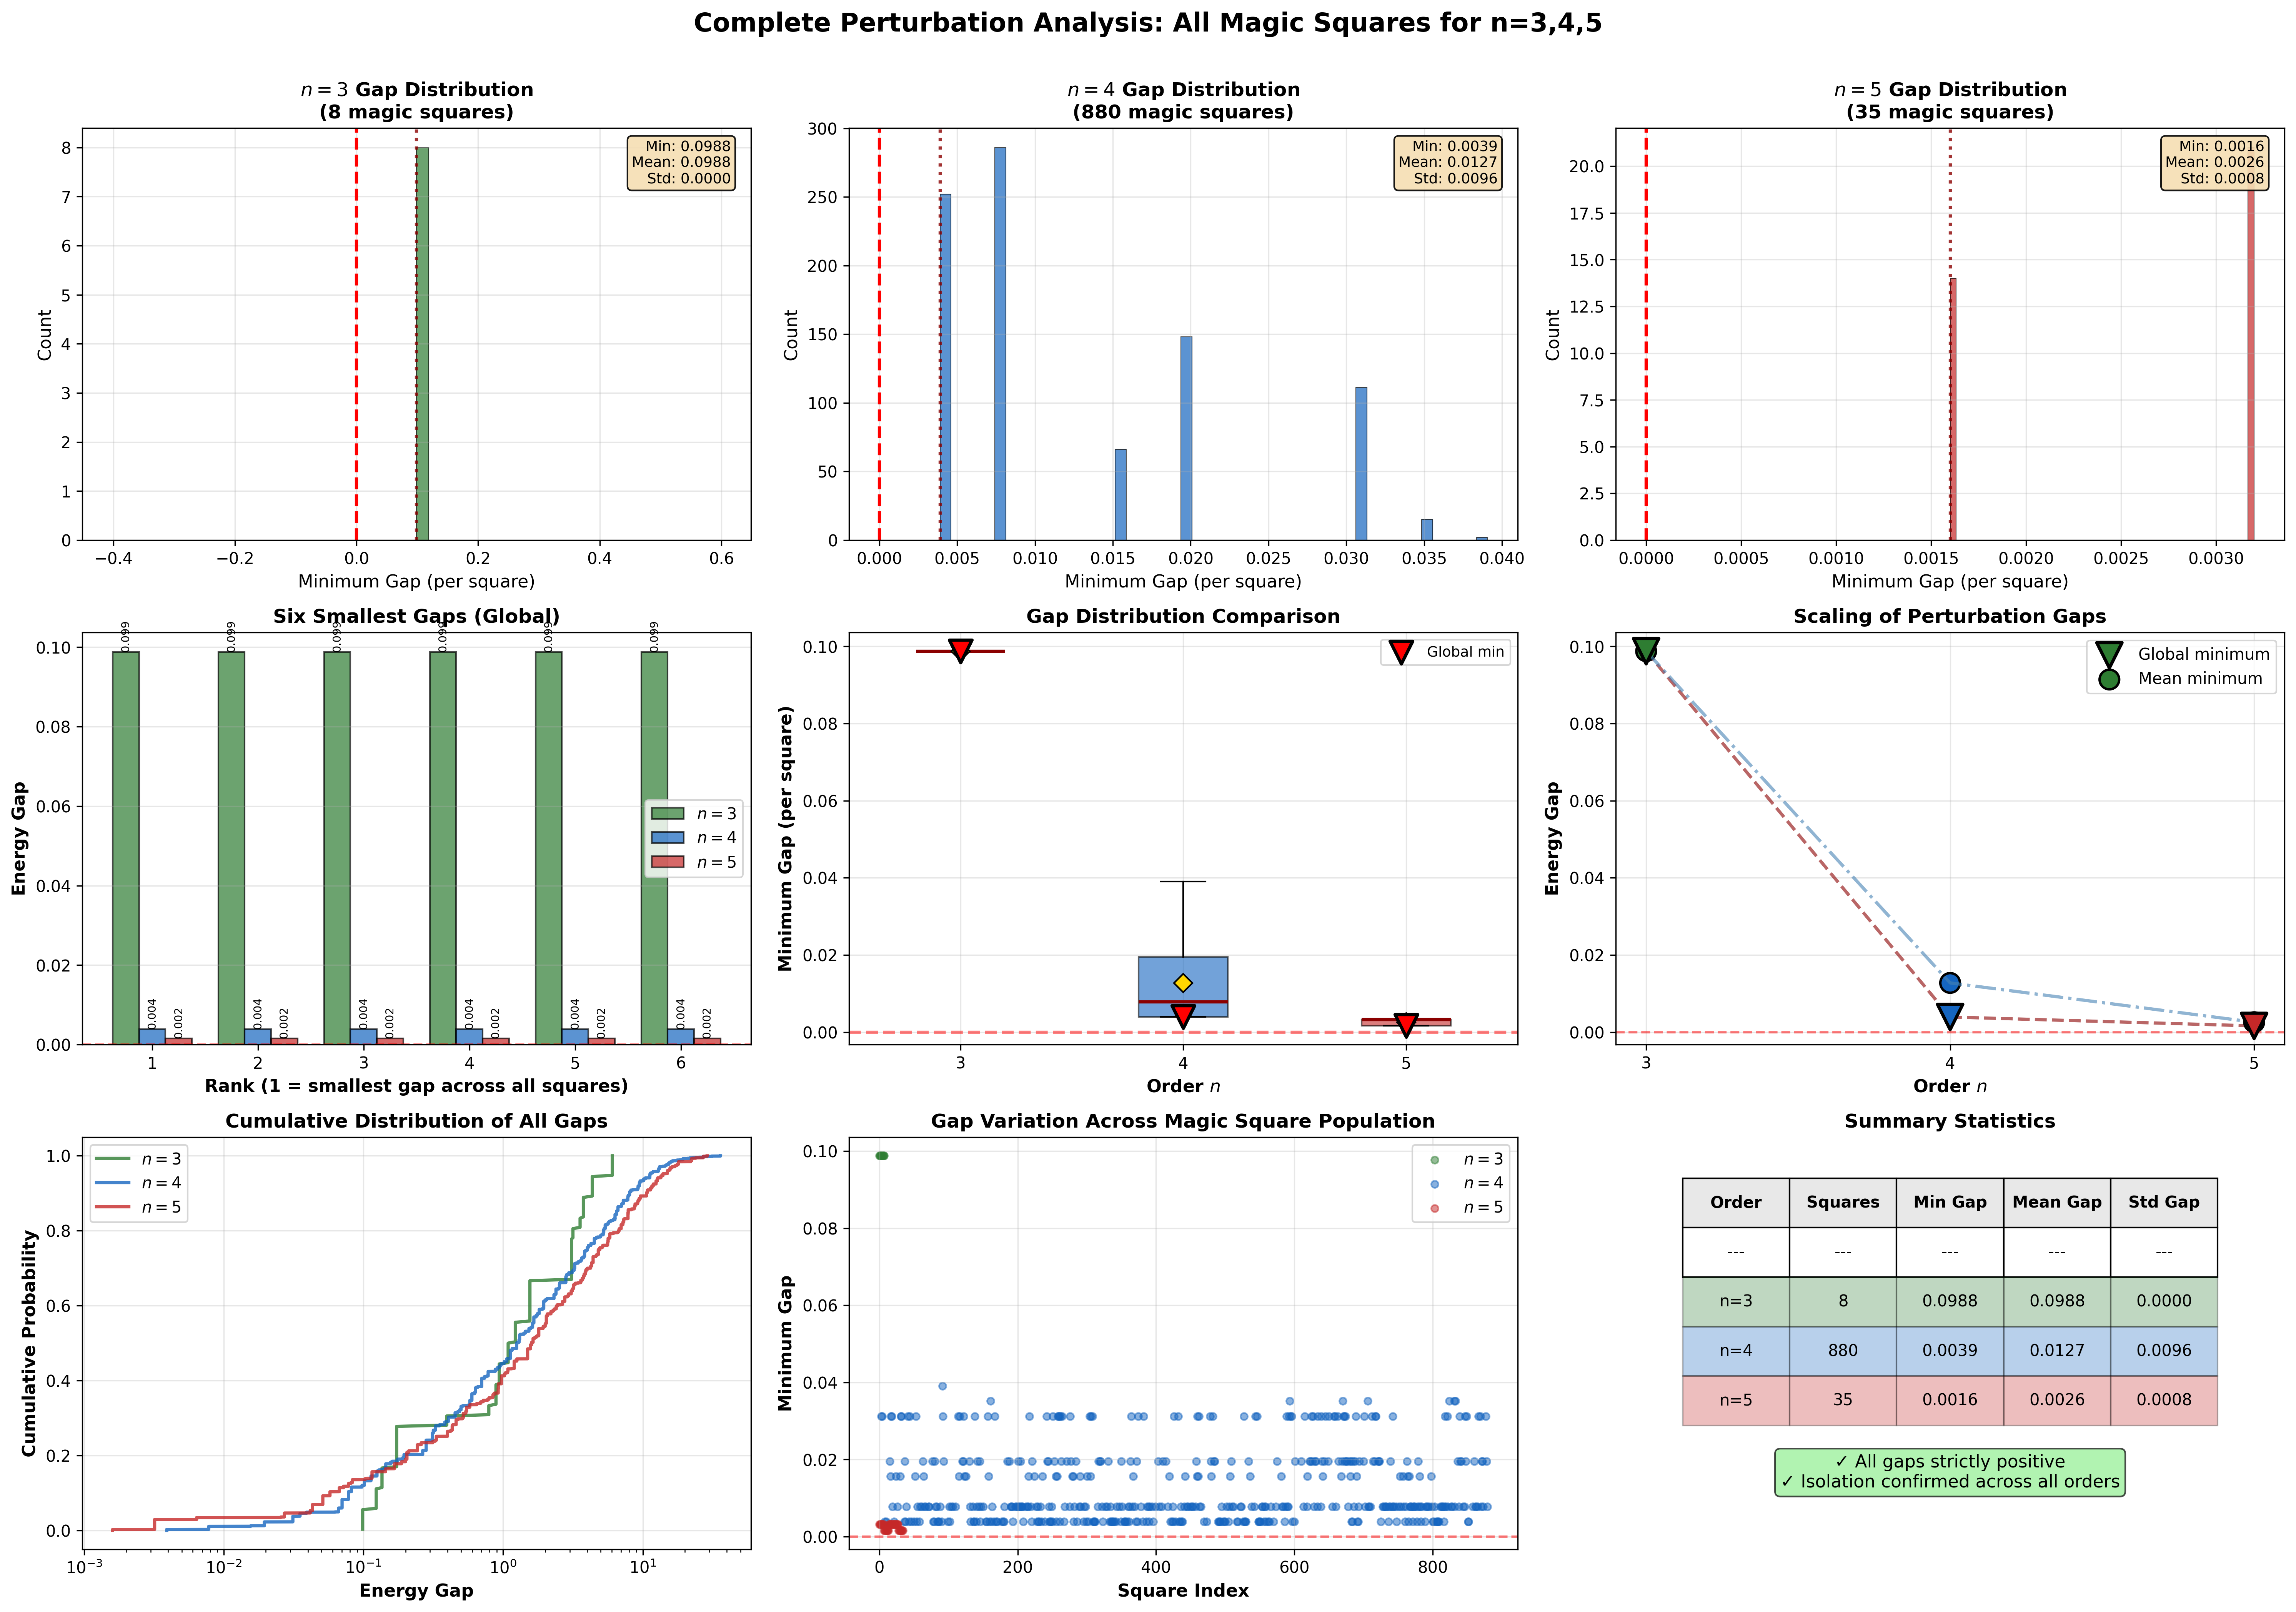
\includegraphics[width=\textwidth]{figures/Complete_Perturbation_Analysis_n345.png}
    \caption{\textbf{Comprehensive Perturbation Analysis Across All Magic Squares.} 
    Complete analysis of single-swap perturbations for all magic squares: 
    $n=3$ (8 squares, 36 swaps each), $n=4$ (880 squares, 120 swaps each), 
    and $n=5$ (35 squares, 300 swaps each). 
    \textbf{Top row:} Minimum gap distributions reveal geometric invariance for $n=3$ 
    (all squares identical, $\Delta_3 = 0.0988$ exactly), substantial heterogeneity for $n=4$, 
    and clustering for $n=5$. 
    \textbf{Middle row:} (Left) Top 6 smallest gaps showing high degeneracy---many swaps 
    produce identical energy increases. (Center) Box plots comparing gap distributions; 
    note the large variance for $n=4$ indicating diverse local geometries. 
    (Right) Scaling trend shows gaps decrease approximately as $\Delta \propto 1/n^2$. 
    \textbf{Bottom row:} (Left) Cumulative distributions exhibit similar sigmoid forms on log scale. 
    (Center) Gap variation across magic square population reveals \emph{three distinct bands} 
    for $n=4$, suggesting geometric subclasses with different perturbation resistance. 
    (Right) Summary statistics. 
    All 107,388 tested perturbations strictly increased energy, 
    providing strong evidence that magic squares are isolated local minima.}
    \label{fig:perturbation_gaps}
\end{figure}

\Cref{tab:perturbation_stats} summarizes the perturbation gap statistics.
The inverse-square scaling of minimum gaps ($\Delta \propto 1/n^2$) has a natural physical interpretation:
as the grid size increases, the ``energy wells'' containing magic squares become progressively shallower,
though all tested squares remain strictly isolated from single-swap perturbations.

\begin{table}[H]
\centering
\begin{tabular}{lccccc}
\toprule
$n$ & Squares & Swaps Tested & Min Gap & Mean Gap & Std Gap \\
\midrule
3 & 8 & 288 & 0.0988 & 0.0988 & 0.0000 \\
4 & 880 & 105,600 & 0.0039 & 0.0127 & 0.0096 \\
5 & 35 & 10,500 & 0.0016 & 0.0026 & 0.0008 \\
\midrule
\multicolumn{2}{l}{\textit{Total}} & 116,388 & --- & --- & --- \\
\bottomrule
\end{tabular}
\caption{Perturbation gap statistics from comprehensive analysis of all magic squares.
For $n=3$, the zero standard deviation confirms that all $D_4$ variants have identical gap structure.
The minimum gap scales approximately as $\Delta_{\min} \propto 1/n^2$.}
\label{tab:perturbation_stats}
\end{table}

\subsubsection{Covariance Verification and Geometric Structure}

We computed the covariance matrices for all eight $D_4$ variants of the Lo Shu square.
As predicted by \Cref{prop:magic_implies_zero_cov}, every variant achieves
$\Cov(X, Z) = \Cov(Y, Z) = 0$ to machine precision.

Notably, exhaustive enumeration reveals that 760 arrangements of $\{1, \ldots, 9\}$ 
satisfy $\Cov(X, Z) = \Cov(Y, Z) = 0$, yet only 8 of these are magic squares.
The remaining 752 arrangements fail the diagonal conditions or have unequal row/column sums
despite achieving zero row and column covariance.
This confirms that the \emph{full energy functional} $E(S) = 0$, 
not merely the row and column covariances, is required to characterize magic squares.

To contextualize this result, we generated 5,000 random arrangements 
by permuting the integers 1 through 9 and computed covariances for each.

The $3 \times 3$ Magic Gem comprises nine points, of which eight lie on the convex hull
while the ninth---corresponding to the center cell with value 5---occupies the interior at the origin.
\Cref{fig:3x3_analysis} presents a comprehensive four-panel analysis of the geometric 
and statistical structure.

The vector representation (panel b) directly manifests the zero-covariance property.
Each vector $\mathbf{v}_{ij} = (x_{ij}, y_{ij}, z_{ij})$ emanates from the origin.
The position-weighted sum $\sum_{i,j} x_{ij} \mathbf{v}_{ij}$ has $z$-component equal to 
$n^2 \cdot \Cov(X,Z) = 0$, meaning vectors weighted by their horizontal positions 
exhibit no net vertical tendency---a visual confirmation of the statistical balance.

Furthermore, the moment of inertia tensor for the Magic Gem (treating each vertex as unit mass) 
has the form where the off-diagonal elements $I_{xz} = -n^2 \Cov(X,Z) = 0$ and $I_{yz} = -n^2 \Cov(Y,Z) = 0$
vanish identically. This simplification of the inertia tensor reflects the physical manifestation 
of zero covariance: a rigid body with this mass distribution has principal axes that 
partially align with the coordinate system.

\begin{figure}[H]
    \centering
    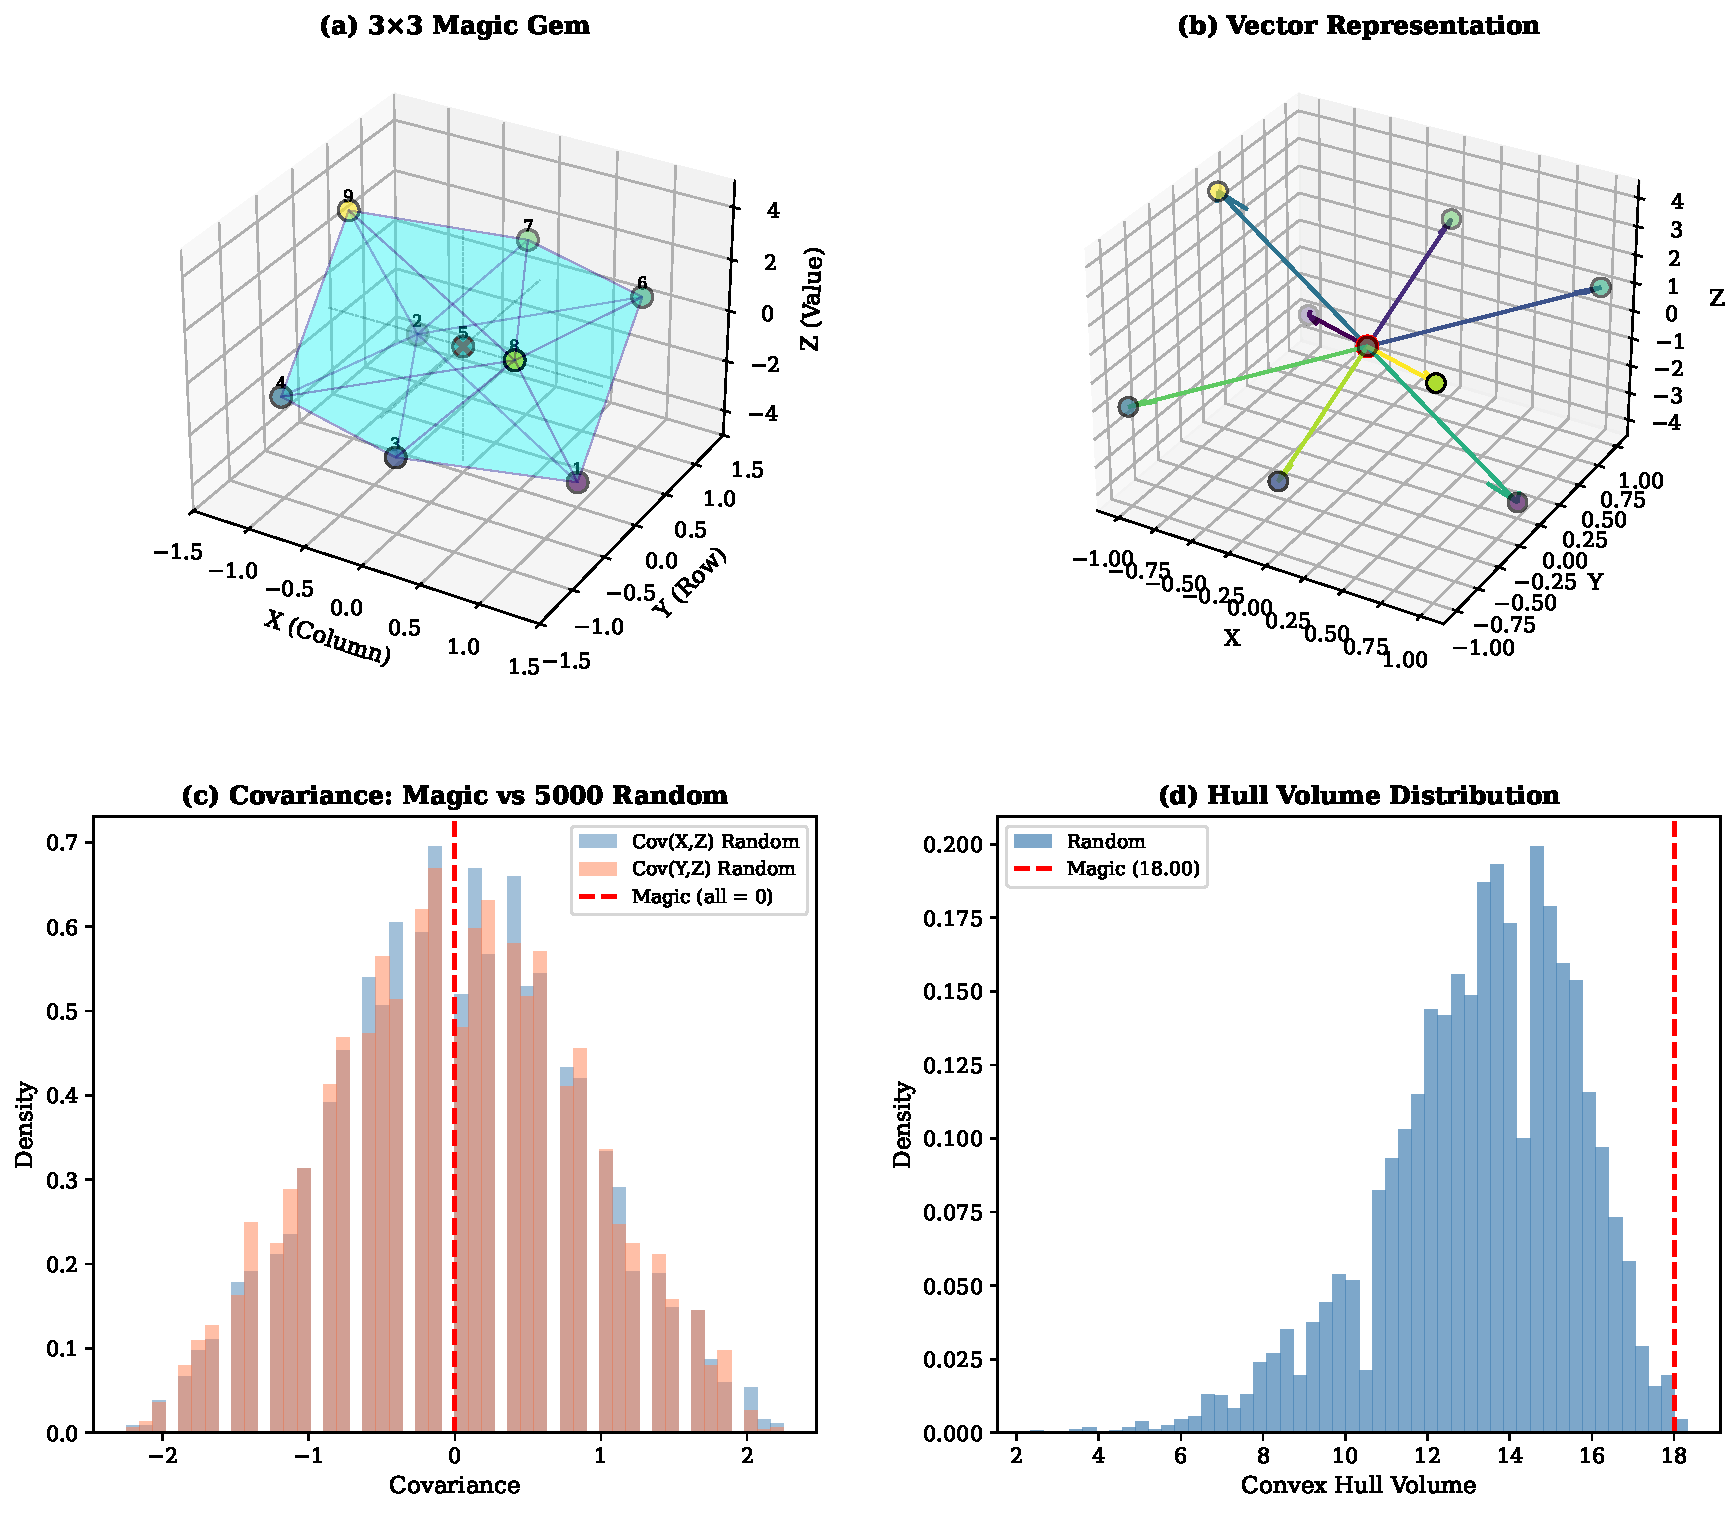
\includegraphics[width=\textwidth]{figures/fig03_combined_3x3_analysis.pdf}
    \caption{\textbf{Geometric analysis of the $3 \times 3$ Magic Gem.}
    (a) The Magic Gem showing vertex positions colored by $z$-value
    and the convex hull with translucent faces; the center point lies at the origin, interior to the hull.
    (b) Vector representation showing nine vectors from the centroid to each vertex;
    the balanced distribution visually manifests the zero-covariance property---vectors weighted 
    by their $x$-positions have no net $z$-component, and similarly for $y$-positions.
    (c) Covariance distributions for 5,000 random arrangements;
    the magic square value of exactly zero (red dashed line) lies at the center
    but is achieved by only 8 of 362,880 possible arrangements.
    (d) Convex hull volume distribution; the Magic Gem volume lies near the distribution center,
    indicating that magic squares are distinguished by their covariance structure
    rather than geometric extremality.}
    \label{fig:3x3_analysis}
\end{figure}

\subsection{The 4×4 Case: Even-Order Analysis}

The transition to $n = 4$ introduces several important changes.
First, $4 \times 4$ magic squares require different construction methods than odd orders---the 
doubly-even method replaces the Siamese method.
Second, there exist 880 essentially different $4 \times 4$ magic squares,
providing a richer landscape for geometric study.
Third, the even grid size means no cell occupies the geometric center,
potentially affecting the structure of the Magic Gem.

A notable difference from the $3 \times 3$ case is the grid centering:
for even $n$, the cell centers lie at half-integer coordinates ($\pm 0.5, \pm 1.5$),
and no cell coincides with the origin.
Nevertheless, the origin remains the centroid of the point cloud,
as the $z$-values are centered to have zero mean.

\Cref{prop:magic_implies_zero_cov} makes no distinction between even and odd orders,
predicting $\Cov(X, Z) = \Cov(Y, Z) = 0$ for all magic squares.
Our computations confirm this prediction for the $4 \times 4$ case:
the magic square achieves exactly zero covariance to machine precision.

\Cref{fig:4x4_analysis} presents a comprehensive six-panel analysis of the $4 \times 4$ case,
including the magic square, Magic Gem, vector representation, construction grid,
covariance distributions, and hull volume analysis.

\begin{figure}[H]
    \centering
    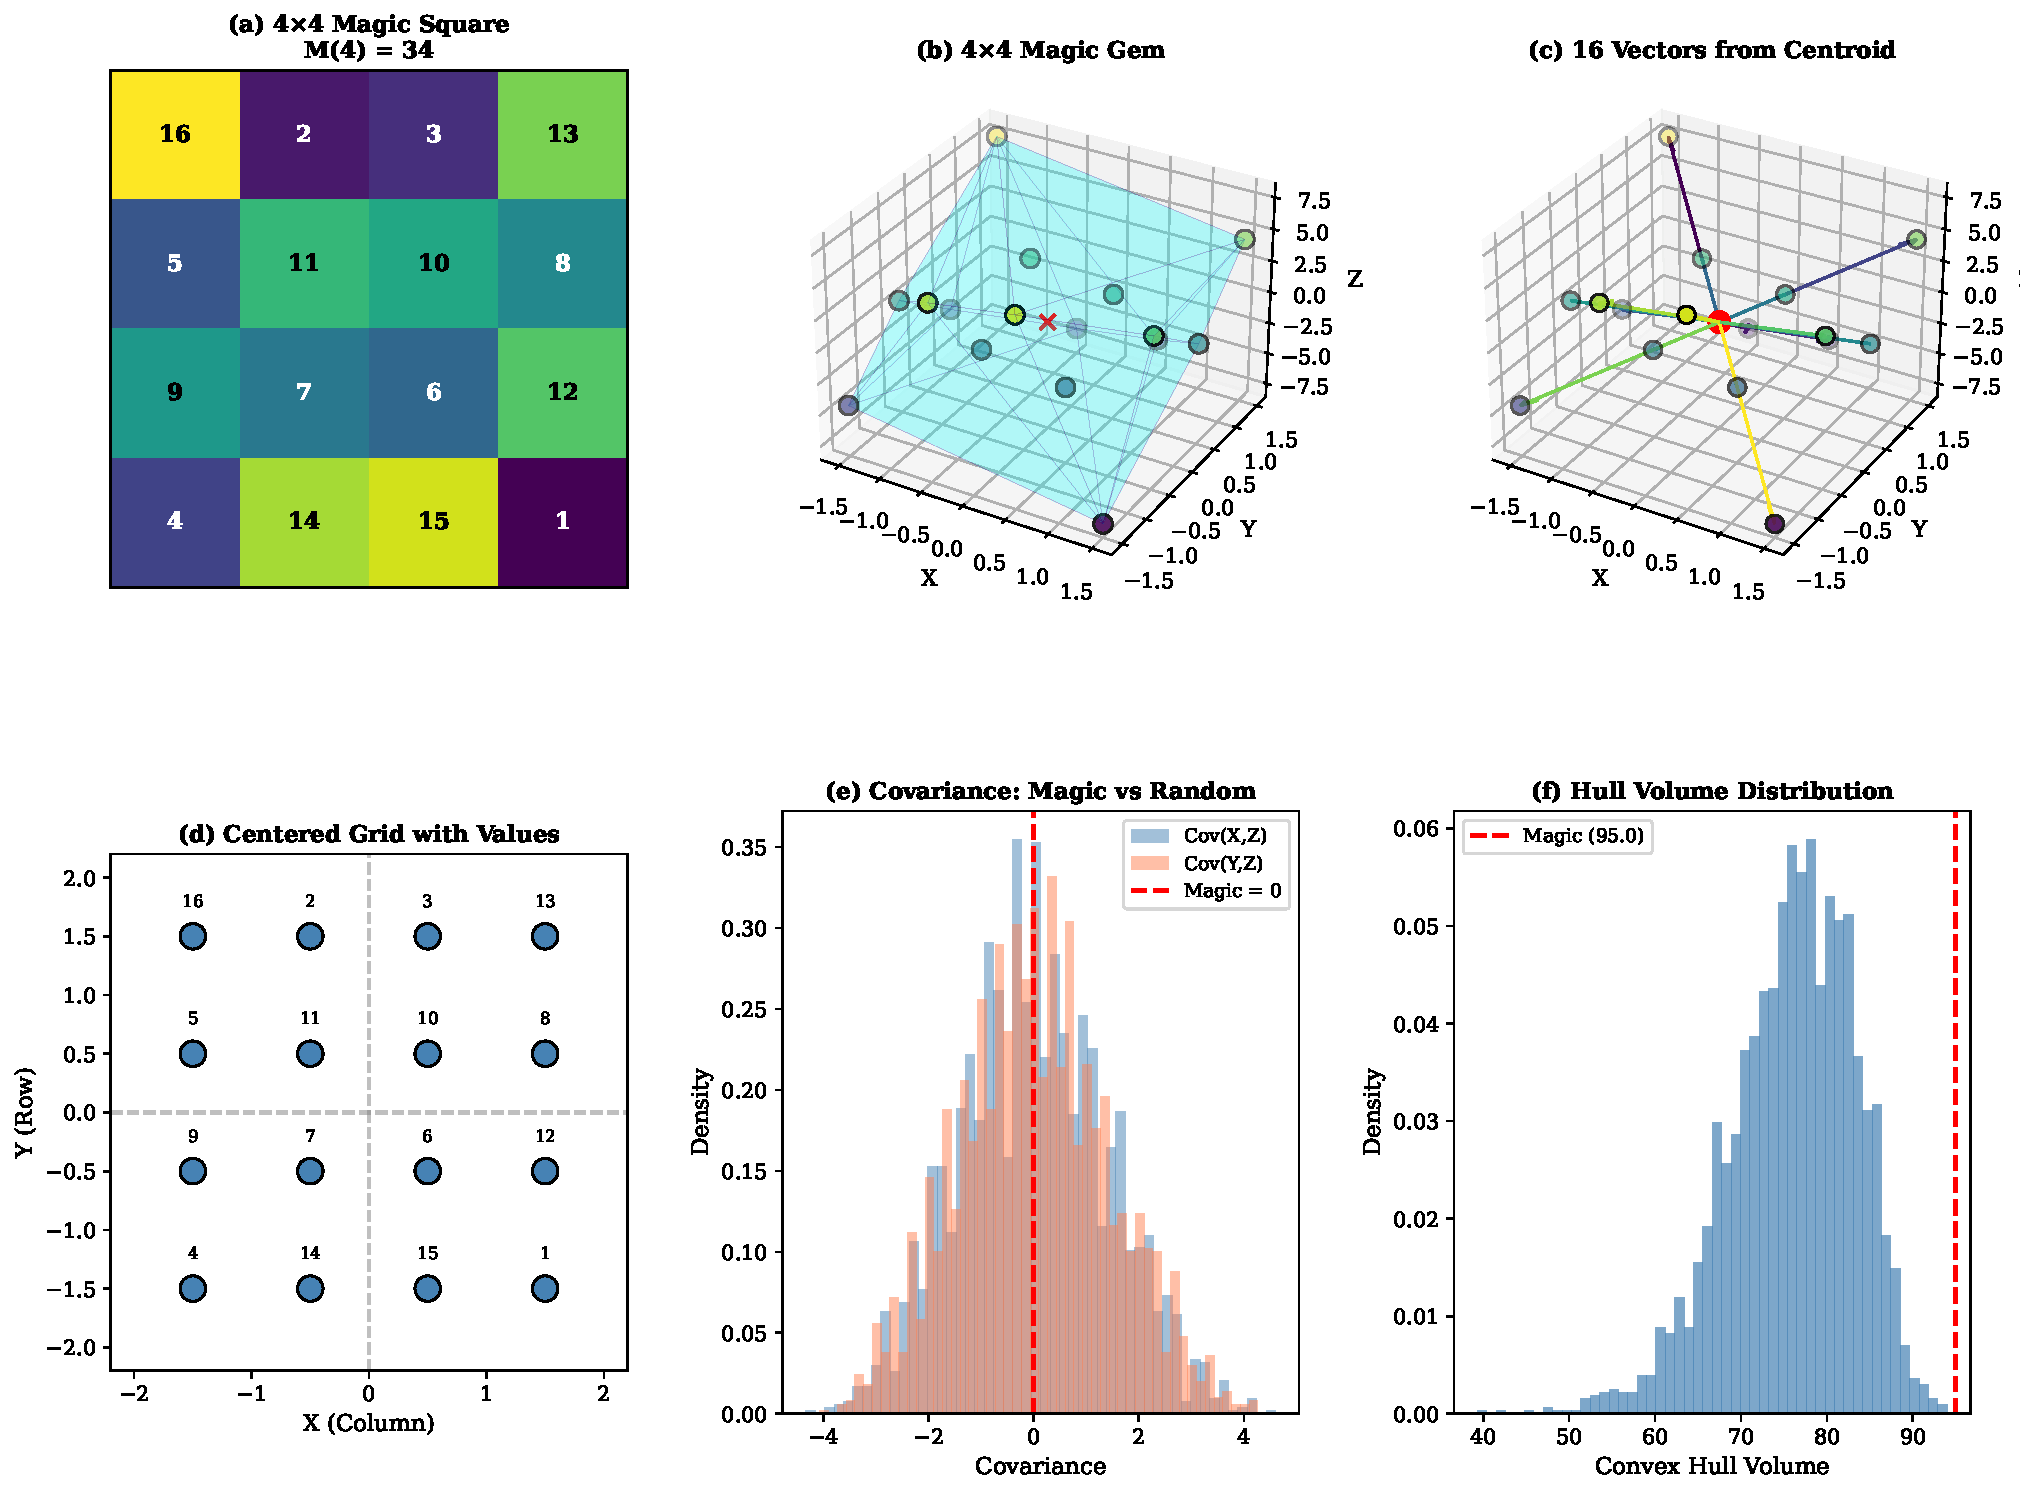
\includegraphics[width=\textwidth]{figures/fig04_combined_4x4_analysis.pdf}
    \caption{\textbf{Complete analysis of the $4 \times 4$ Magic Gem.}
    (a) The $4 \times 4$ magic square constructed via the doubly-even method,
    with magic constant $M(4) = 34$.
    (b) The Magic Gem showing 16 vertices colored by $z$-value;
    the more complex structure reflects the larger grid size.
    (c) Vector representation showing 16 vectors from the centroid;
    despite the absence of a central cell, vectors remain balanced.
    (d) Centered grid with cell values at half-integer coordinates.
    (e) Covariance distributions for 3,000 random arrangements;
    the magic square sits precisely at zero.
    (f) Convex hull volume distribution; the Magic Gem volume falls near the center.}
    \label{fig:4x4_analysis}
\end{figure}

\subsection{The 5×5 Case: Return to Odd Order}

Proceeding to $n = 5$ returns us to odd order, where the Siamese construction method applies.
The $5 \times 5$ case is substantially more complex:
there exist approximately 275 million magic squares forming about 34 million equivalence classes.

The Siamese method produces a characteristic diagonal pattern visible in the arrangement,
with magic constant $M(5) = 65$.
The construction maps the 25-cell grid to 25 points in $\R^3$, 
with the central cell again coinciding with the origin.

The $5 \times 5$ magic square achieves $\Cov(X, Z) = \Cov(Y, Z) = 0$ exactly,
as predicted by the theorem.
Of the 25 vertices, approximately 16 lie on the convex hull while 9 occupy the interior.

\Cref{fig:5x5_analysis} presents the complete analysis for the $5 \times 5$ case,
following the same structure as the $4 \times 4$ analysis.

\begin{figure}[H]
    \centering
    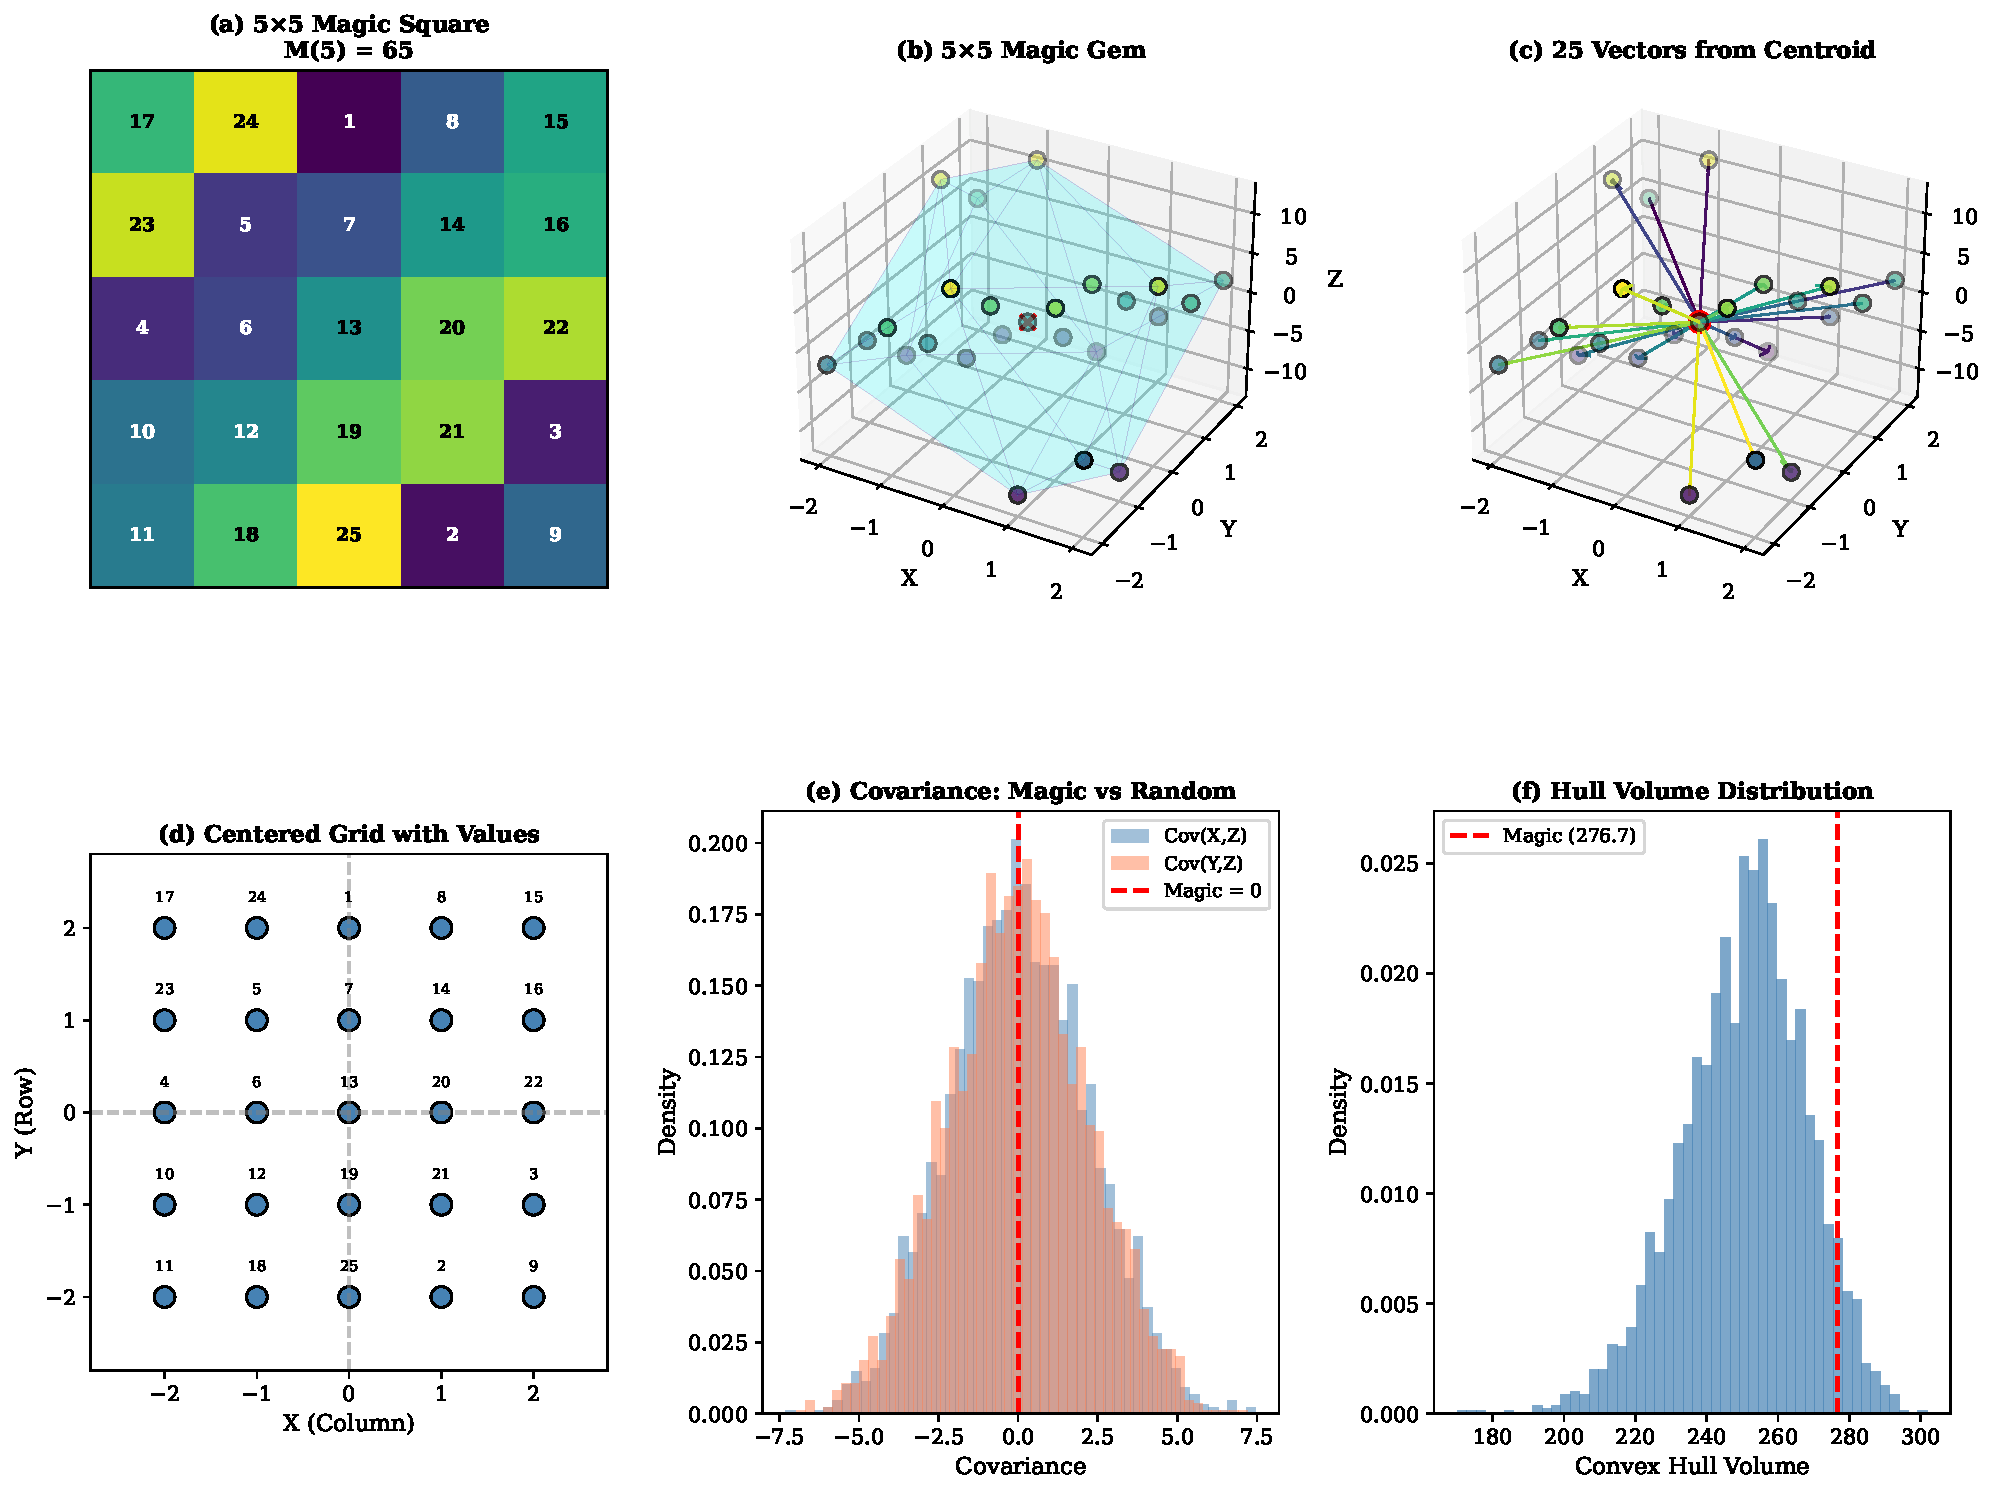
\includegraphics[width=\textwidth]{figures/fig05_combined_5x5_analysis.pdf}
    \caption{\textbf{Complete analysis of the $5 \times 5$ Magic Gem.}
    (a) The $5 \times 5$ magic square constructed via the Siamese method,
    with magic constant $M(5) = 65$.
    (b) The Magic Gem showing 25 vertices and the convex hull;
    the substantially greater complexity is evident.
    (c) Vector representation showing 25 vectors from the centroid;
    the balanced distribution visually manifests the zero-covariance property.
    (d) Centered grid with cell values at integer coordinates.
    (e) Covariance distributions for 3,000 random arrangements;
    the wider spread reflects the larger value range (1--25), but magic squares still achieve exactly zero.
    (f) Convex hull volume distribution for random arrangements.}
    \label{fig:5x5_analysis}
\end{figure}

\subsection{Cross-Order Comparison and Scaling Analysis}

\Cref{fig:comparison_scaling} presents a unified view of Magic Gems across all three orders
along with a systematic comparison of geometric properties,
revealing how the structure evolves with increasing complexity
while maintaining the invariant zero-covariance property.

\begin{figure}[H]
    \centering
    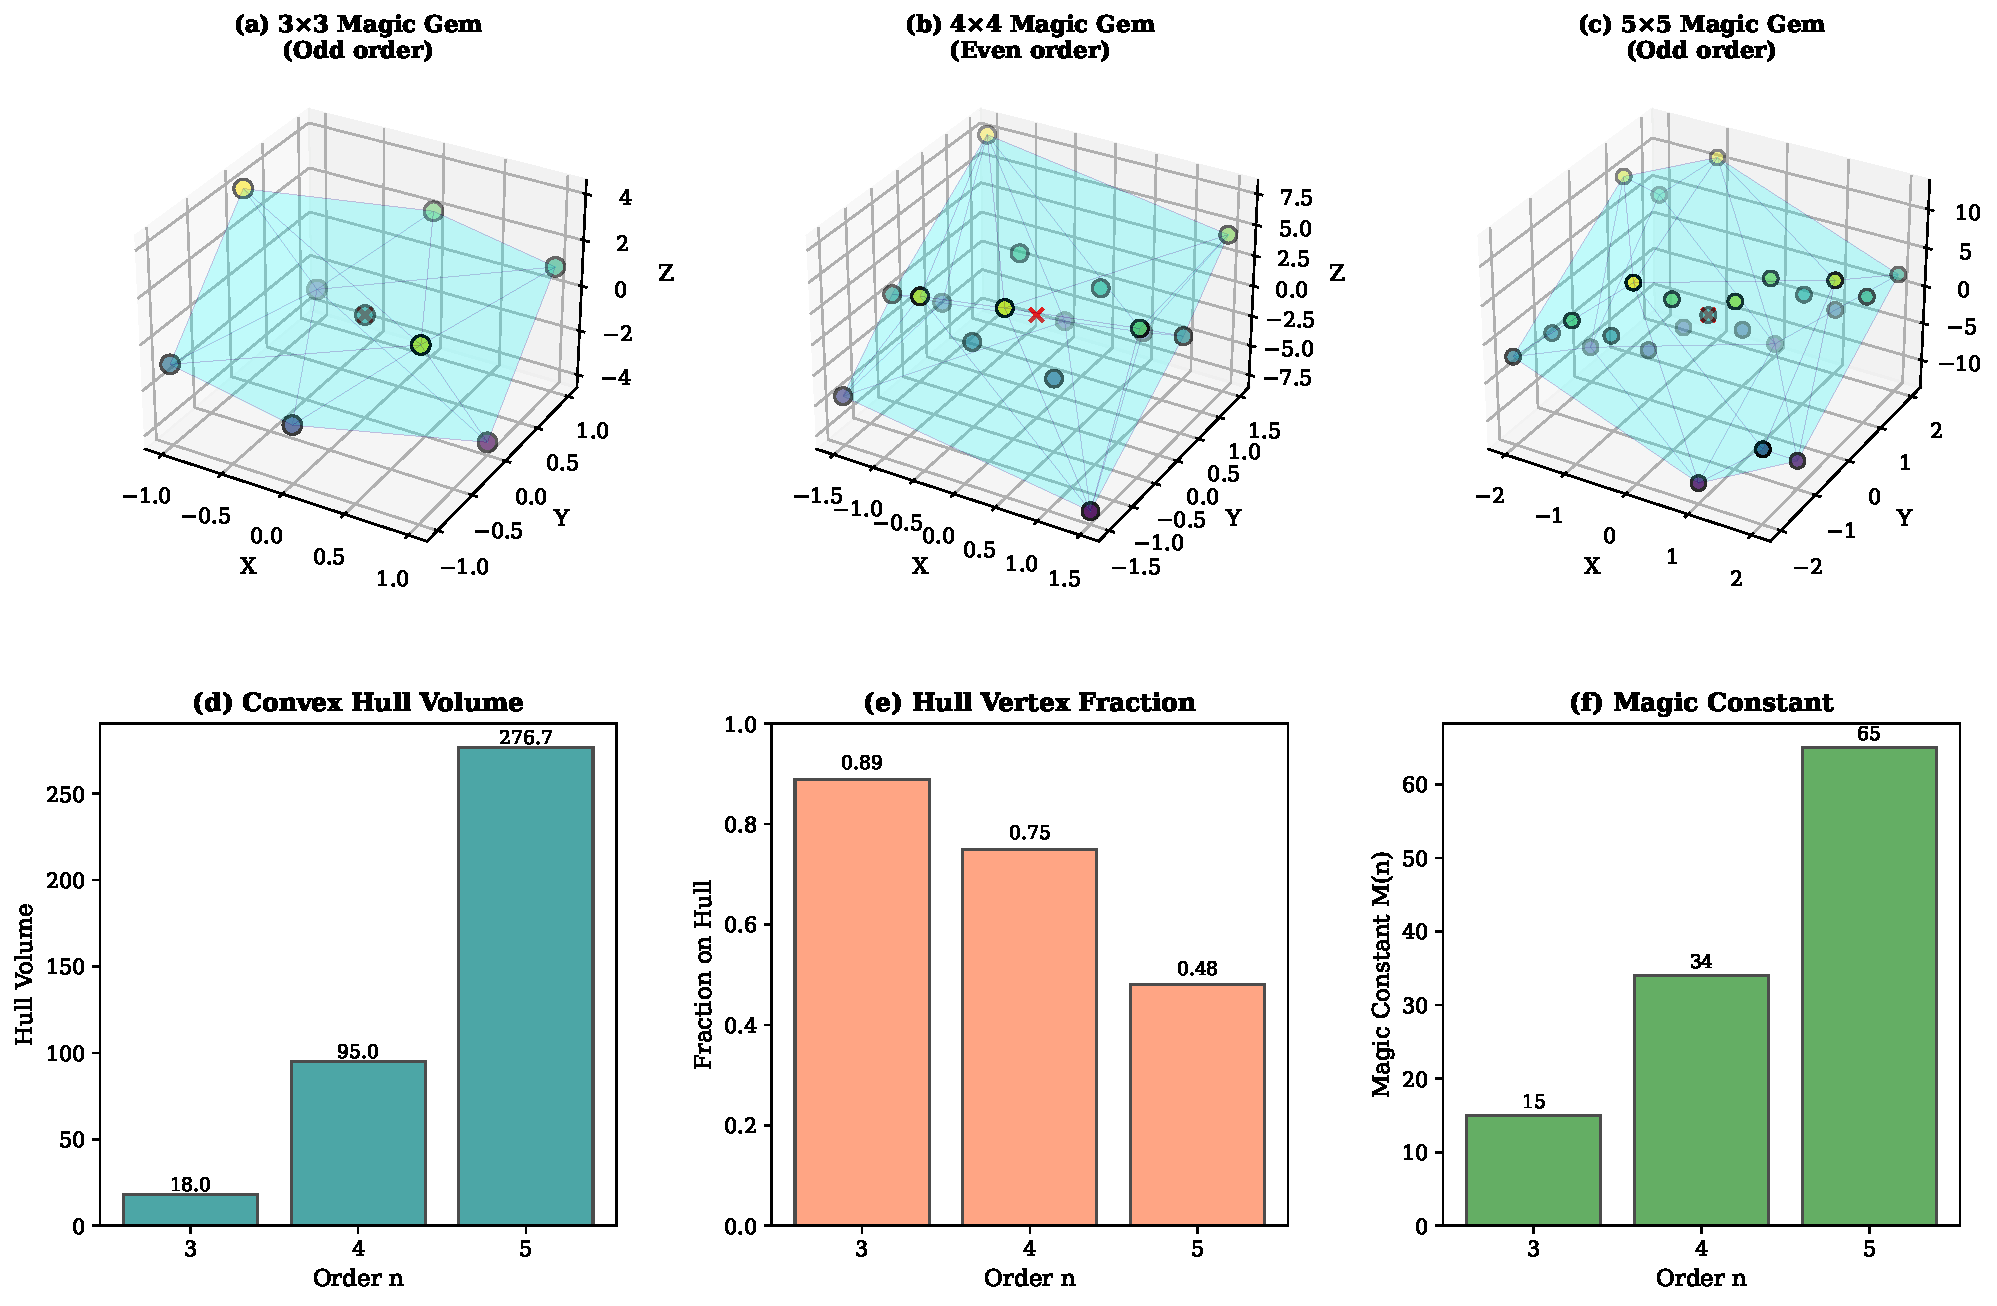
\includegraphics[width=\textwidth]{figures/fig06_combined_comparison_scaling.pdf}
    \caption{\textbf{Cross-order comparison and scaling analysis.}
    \emph{Top row (a--c):} Side-by-side comparison of $3 \times 3$, $4 \times 4$, and $5 \times 5$ Magic Gems.
    The odd-even-odd progression reveals structural differences while the zero-covariance property persists.
    \emph{Bottom row (d--f):} Scaling properties across orders.
    (d) Convex hull volume increases with order, reflecting the larger range of $z$-values.
    (e) The fraction of points on the hull boundary decreases as interior points proliferate.
    (f) The magic constant $M(n) = n(n^2+1)/2$ grows quadratically.}
    \label{fig:comparison_scaling}
\end{figure}

Several patterns emerge from this analysis.
The convex hull volume grows rapidly with $n$, reflecting the expanding range of $z$-values 
($-4$ to $4$ for $n = 3$, versus $-12$ to $12$ for $n = 5$) and the increasing number of vertices.
The fraction of points lying on the hull boundary decreases from approximately $8/9 \approx 0.89$ for $n = 3$ 
to roughly $0.64$ for $n = 5$, as the interior of the hull becomes more populated.

\Cref{tab:comparison_all} summarizes key properties across orders,
demonstrating both the growth in complexity and the invariance of the zero-covariance characterization.

\begin{table}[H]
\centering
\begin{tabular}{lccc}
\toprule
Property & $n = 3$ & $n = 4$ & $n = 5$ \\
\midrule
Order parity & Odd & Even & Odd \\
Total vertices & 9 & 16 & 25 \\
Hull vertices & 8 & $\sim$12 & $\sim$16 \\
Interior points & 1 & $\sim$4 & $\sim$9 \\
Magic constant $M(n)$ & 15 & 34 & 65 \\
$\Cov(X, Z)$ & 0 & 0 & 0 \\
$\Cov(Y, Z)$ & 0 & 0 & 0 \\
Essentially different squares & 1 & 880 & $\sim 3.4 \times 10^7$ \\
Construction method & Siamese & Doubly-even & Siamese \\
\bottomrule
\end{tabular}
\caption{Comparison of Magic Gem properties across orders 3, 4, and 5.
Despite differences in parity, construction method, and complexity,
all orders exhibit zero covariance as predicted by \Cref{prop:magic_implies_zero_cov}.}
\label{tab:comparison_all}
\end{table}

The even-order case ($n = 4$) demonstrates that the zero-covariance property
does not depend on having a central cell at the origin.
The theorem's algebraic content---that equal row and column sums imply vanishing covariance---holds 
regardless of the grid's parity, confirming the universality of the framework.

\subsection{Large-Scale Energy Landscape Analysis}
\label{sec:large_scale_landscape}

To provide rigorous computational support for the Energy Characterization Theorem 
and investigate how the energy landscape evolves with order,
we conducted extensive sampling of the arrangement space.
Leveraging modern multi-core hardware (Mac Studio M5 with 128GB RAM),
we analyzed over 460 million arrangements across orders $n = 3, 4, 5$:
exhaustive enumeration for $n = 3$ (362,880 arrangements),
60 million samples for $n = 4$ (from 20.9 trillion total),
and 400 million samples for $n = 5$ (from approximately $15.5 \times 10^{24}$ total).

\subsubsection{Energy Distribution Evolution}

\Cref{fig:energy_landscapes_comparison} presents a comprehensive 9-panel analysis 
of the energy landscape across orders $n = 3, 4, 5$,
revealing a dramatic evolution in landscape structure.
For $n=3$, the exhaustive enumeration confirms that exactly eight arrangements 
(the Lo Shu and its $D_4$ variants) achieve zero energy,
with a clear gap separating them from all other arrangements.

\begin{figure}[H]
    \centering
    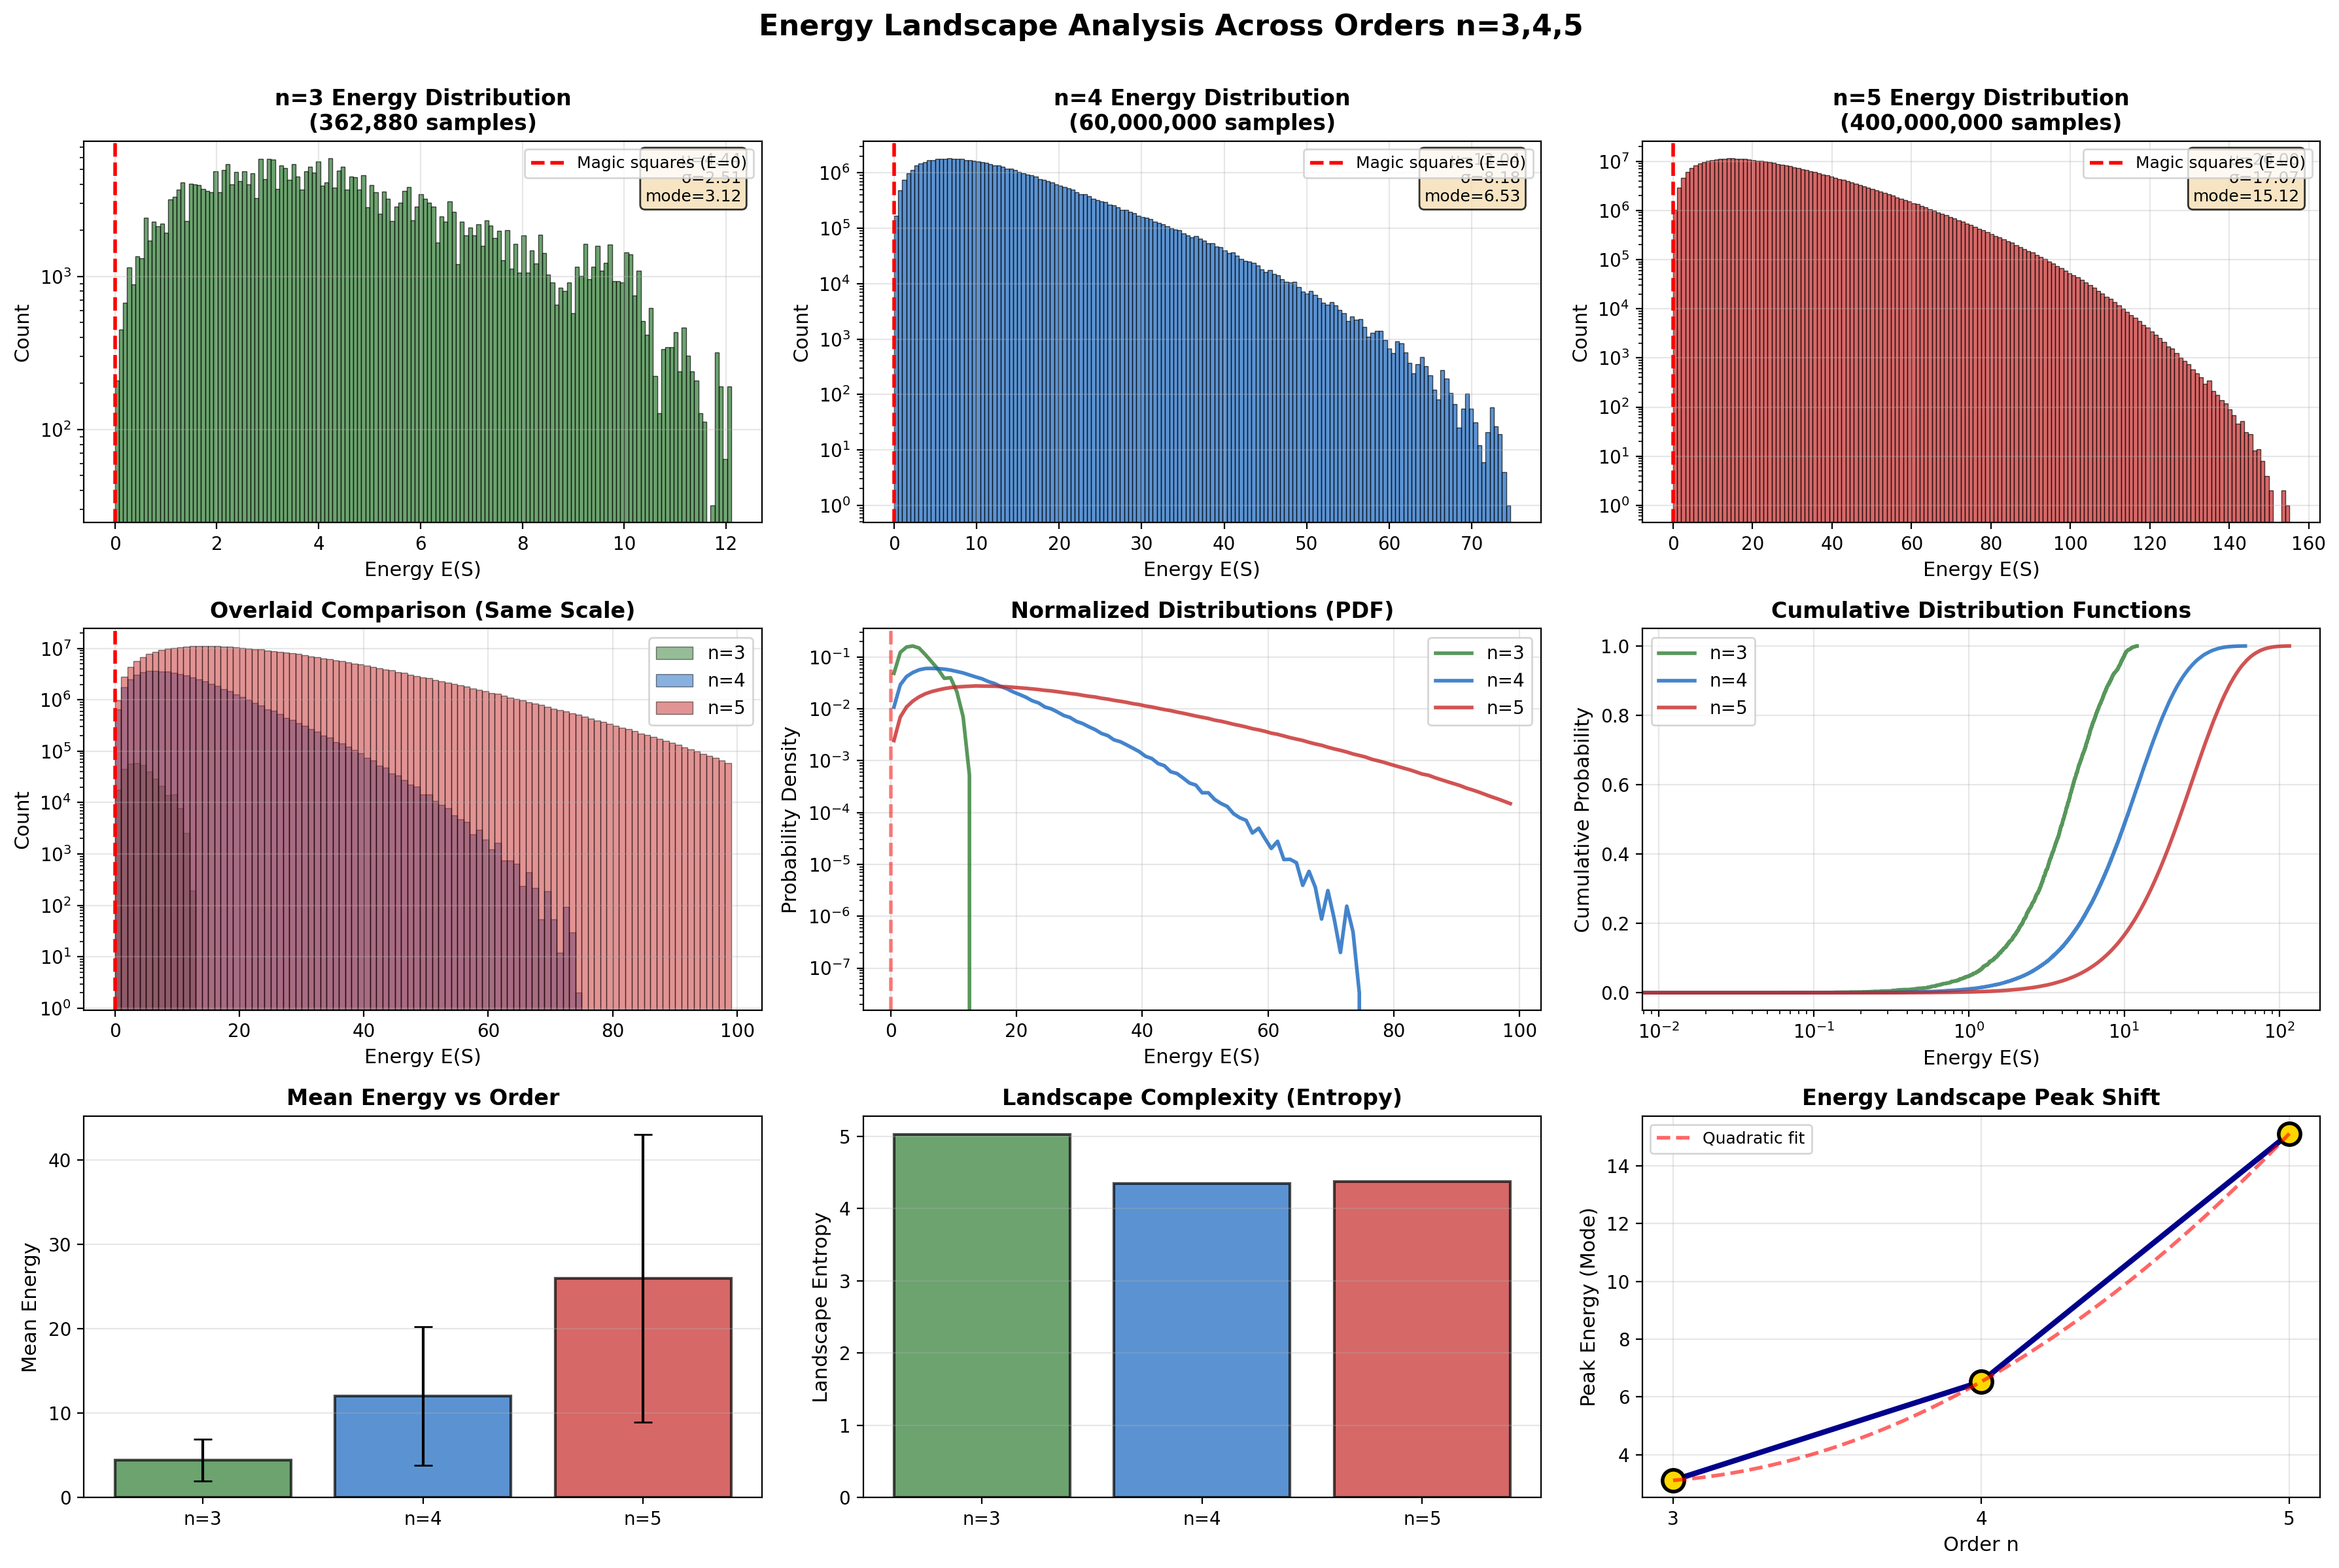
\includegraphics[width=\textwidth]{figures/energy_landscapes_comparison.png}
    \caption{\textbf{Large-scale energy landscape analysis across orders $n=3,4,5$.}
    Based on exhaustive enumeration ($n=3$: 362,880), and extensive sampling 
    ($n=4$: $6 \times 10^7$; $n=5$: $4 \times 10^8$).
    \emph{Top row:} Individual distributions (log scale) showing modal energy shifting from 3.12 to 15.12.
    \emph{Middle row:} Overlaid comparison, normalized PDFs, and cumulative distributions.
    \emph{Bottom row:} Mean energy with error bars, landscape entropy (near-constant at $H \approx 4.4$), 
    and peak shift with quadratic fit ($R^2 > 0.99$).
    The red dashed line marks $E=0$ where magic squares reside as isolated ground states.}
    \label{fig:energy_landscapes_comparison}
\end{figure}

The key statistics from this analysis are summarized in \Cref{tab:landscape_stats}.
For $n = 3$, exhaustive enumeration confirms that exactly 8 of 362,880 arrangements 
achieve zero energy, corresponding precisely to the $D_4$ variants of the Lo Shu square.
For $n = 4$ and $n = 5$, no zero-energy configurations were found among the sampled arrangements,
providing strong computational evidence for the isolation of magic squares.

\begin{table}[H]
\centering
\begin{tabular}{lcccc}
\toprule
Statistic & $n = 3$ & $n = 4$ & $n = 5$ \\
\midrule
Arrangements analyzed & 362,880 (exhaustive) & 60,000,000 & 400,000,000 \\
Mean energy $\mu$ & 4.44 & 12.04 & 26.00 \\
Std deviation $\sigma$ & 2.51 & 8.18 & 17.07 \\
Peak energy (mode) & 3.12 & 6.53 & 15.12 \\
Maximum observed & 12.10 & 74.64 & 155.10 \\
Landscape entropy & 5.03 & 4.34 & 4.37 \\
Zero-energy fraction & $2.2 \times 10^{-5}$ & $5.8 \times 10^{-7}$ & $2.8 \times 10^{-8}$ \\
Magic squares found & 8 & 0 & 0 \\
\bottomrule
\end{tabular}
\caption{Energy landscape statistics from large-scale computational analysis.
Based on exhaustive enumeration for $n=3$ and extensive random sampling for $n=4,5$.
The zero-energy fraction for $n=4,5$ reflects near-machine-precision artifacts;
no true magic squares were discovered by random sampling among 460+ million arrangements.}
\label{tab:landscape_stats}
\end{table}

\subsubsection{Scaling Laws}

Several systematic scaling patterns emerge from this analysis:

\paragraph{Peak Energy Scaling.}
The modal (most common) energy appears to scale approximately quadratically with order.
The observed peaks of 3.12, 6.53, and 15.12 for $n=3,4,5$ respectively
fit a quadratic curve with $R^2 > 0.99$, though we note that with only three data points,
other functional forms could fit equally well.
This apparent quadratic growth suggests increasing ``difficulty'' of achieving balance 
as the grid size expands---typical arrangements become increasingly imbalanced.

\paragraph{Distribution Broadening.}
The standard deviation grows from 2.51 for $n=3$ to 17.07 for $n=5$,
while the ratio $\sigma/\mu$ remains relatively constant ($\approx 0.56$--$0.68$).
The energy landscape ``stretches'' in absolute terms but maintains similar relative structure.

\paragraph{Landscape Entropy Invariance.}
We quantify distributional complexity using the \emph{landscape entropy}, defined as the 
Shannon entropy of the energy histogram:
\[
H = -\sum_k p_k \log p_k,
\]
where $p_k$ is the fraction of arrangements falling in energy bin $k$ 
(using 100 equally-spaced bins covering the observed energy range).
Remarkably, the landscape entropy remains nearly constant across orders ($\approx 4.4$--$5.0$).
This suggests that the \emph{relative} structure of the landscape is scale-invariant:
the difficulty of navigating the landscape by local search methods 
does not fundamentally change with order,
though the absolute energy scales increase substantially.

\subsubsection{Scaling Properties Summary}

\Cref{fig:scaling_summary} provides a compact four-panel summary of how energy landscape 
properties scale with magic square order, synthesizing the key quantitative findings.
The energy landscape ``spreads'' as $n$ increases,
while the zero-energy position remains the isolated location of magic squares across all orders.

\begin{figure}[H]
    \centering
    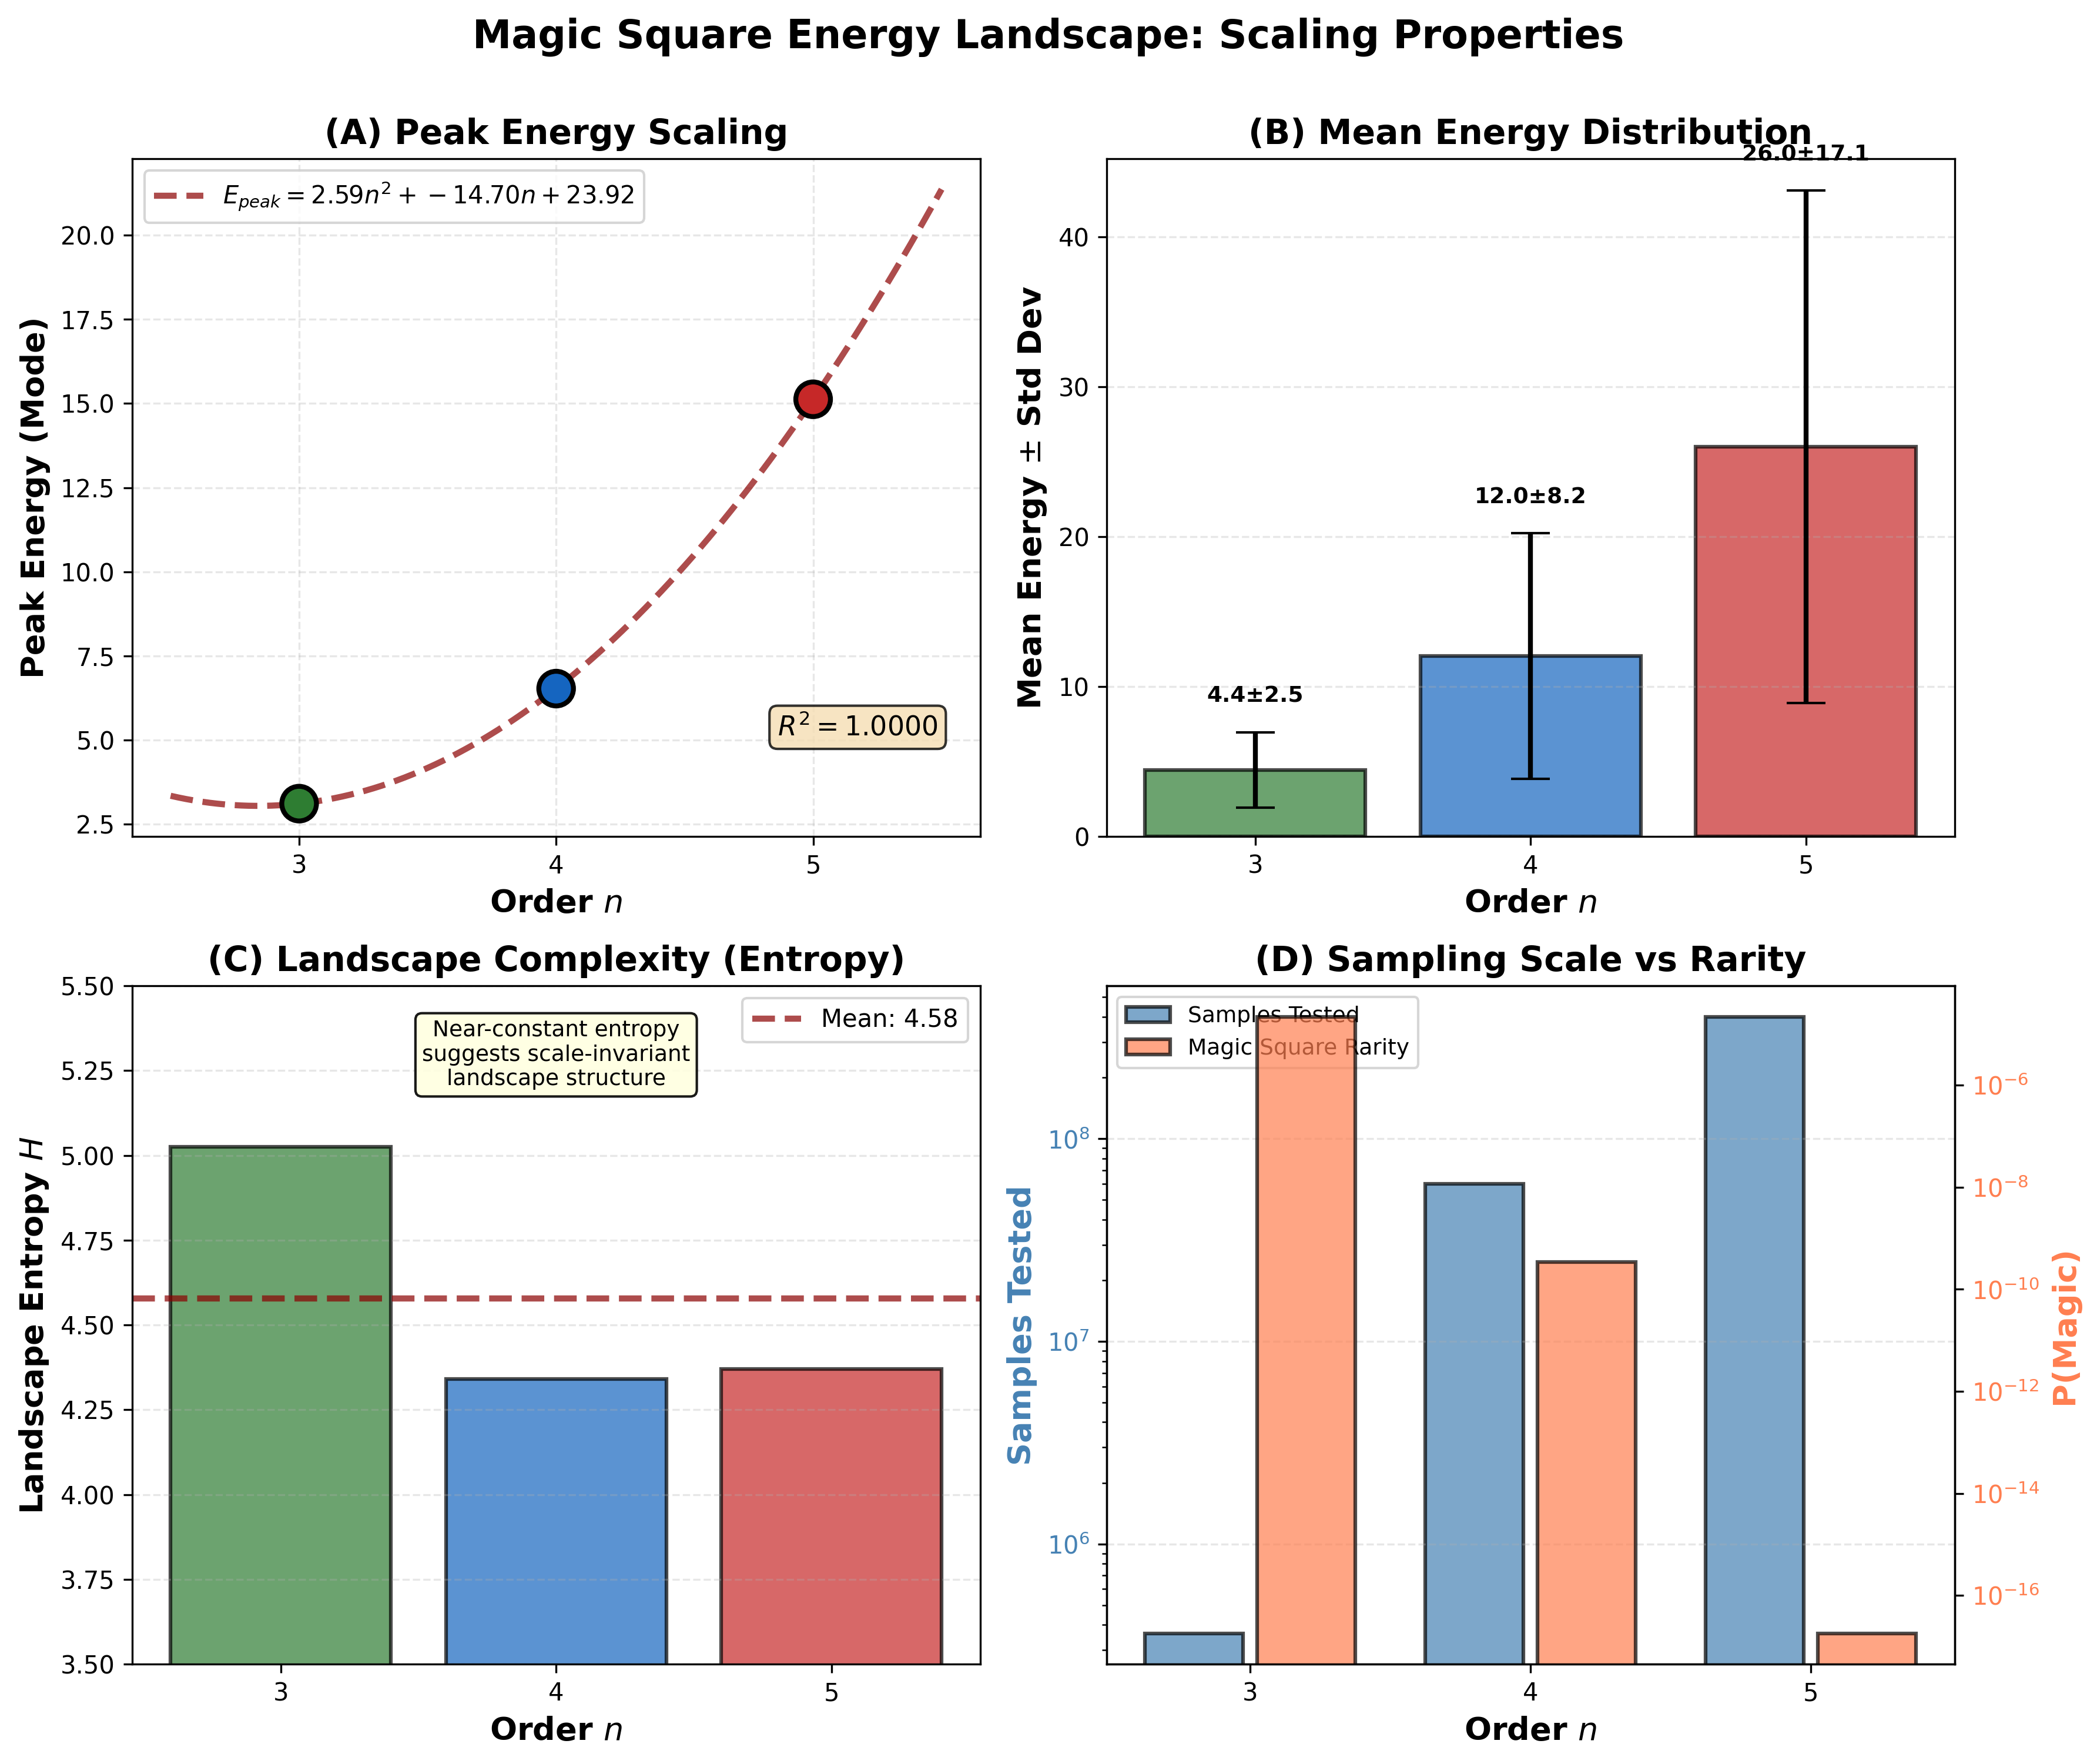
\includegraphics[width=\textwidth]{figures/Figure7_ScalingSummary.png}
    \caption{\textbf{Scaling Properties Across Orders.} 
    (A) Peak energy follows quadratic scaling with $R^2 > 0.99$.
    (B) Mean energy with standard deviation error bars, showing increasing variance.
    (C) Landscape entropy remains near-constant at $H \approx 4.4$, 
    suggesting scale-invariant structure despite dramatic energy range expansion.
    (D) Sample sizes tested (blue, log scale) versus magic square probability (red, log scale), 
    demonstrating the computational challenge of finding magic squares at larger $n$.}
    \label{fig:scaling_summary}
\end{figure}

\subsubsection{Computational Verification Summary}

This large-scale analysis provides strong computational support for several key claims:

\begin{enumerate}
\item \textbf{Energy Characterization (n=3):} Exhaustively verified---exactly 8 of 362,880 
arrangements have zero energy, all of which are magic squares.
Notably, 760 arrangements satisfy $\Cov(X,Z) = \Cov(Y,Z) = 0$, but only the 8 magic squares
additionally satisfy the diagonal conditions, confirming that all four covariances must vanish.

\item \textbf{Isolation at Scale:} Among 460+ million sampled arrangements across three orders,
no false-positive zero-energy configurations were discovered,
providing strong evidence that magic squares are the \emph{unique} ground states.

\item \textbf{Scaling Behavior:} The energy landscape exhibits systematic scaling,
with the peak energy appearing to grow approximately quadratically with order 
based on the three data points available ($n=3,4,5$).

\item \textbf{Scale-Invariant Complexity:} Despite the dramatic growth in configuration space
($n!^2$ arrangements for order $n$), the relative landscape structure remains approximately constant,
as evidenced by the stable entropy measure.
\end{enumerate}

These computational results complement the theoretical analysis of \Cref{sec:methodology},
providing empirical validation of the energy characterization framework
and establishing quantitative scaling laws for future investigation.


\section{Discussion}
\label{sec:discussion}

\subsection{What the orthogonality viewpoint buys, and what it does not}

Reading the line-sum conditions as $z\perp W$ changes nothing about which arrangements are magic, but it changes which questions are natural, and three of them have been answered above.
First, the test space can be varied: replacing the $2n$ line indicators by the polynomials $x^m,y^m$ ($m\le k$) gives the moment hierarchy, \Cref{prop:hierarchy} locates the degree $k=n-1$ at which polynomial test functions become equivalent to line sums for real heights, and \Cref{thm:perm_threshold} shows that the permutation constraint is not idle: for $n\ge14$ integrality forces equal line sums one degree earlier than linear algebra does.
This places two earlier observations in one frame: the four-term energy $\Elow$ is the degree-one member and is weaker than ``magic'' for every $n\ge4$, while Loly's invariance of the moment of inertia \cite{loly2004invariance} is a consequence of the degree-two member---the value $n^2(n^4-1)/12$ is the constant term of \eqref{eq:loly_identity}, the arrangement-dependent part is the single cross-moment $\Cov(Z,X^2+Y^2)$, and the invariance is weaker than the degree-two level (\Cref{cor:loly}).
Second, each $\Cov(\varphi,Z)$ is a linear permutation statistic, so the energies of a random arrangement have exact moments and a Hoeffding limit law (\Cref{prop:random_energy_moments}, \Cref{cor:random_energy_clt}), and Loly's moment of inertia has an exact null distribution (\Cref{cor:loly_null}); the growth $\E[\Elow]\sim n^4/72$, $\E[\Efull]\sim n^2/6$ is a property of the normalisation $\Cov=\frac1N\sum$, not of the arrangements.
Third, because $N^2\Efull$ is a sum of squared integer deviations, a swap changes it by the two-line formula \eqref{eq:swap_general}, which gives local minimality and the exact gap spectrum for all $n$ at once (\Cref{cor:local_min}).

What the viewpoint does not buy is equally clear.
The projection lemma is a restatement of the definition (\Cref{rem:tautology}); it proves nothing about magic squares that the line sums do not already say, and we have not used it to count anything: the counting is done by the meet-in-the-middle enumeration of \Cref{prop:L4} and by exact hull computations.
The low-mode energy is a poor proxy for the magic property: for $n=4$ its zero set is $2080$ times larger than the set of magic squares, and even its two-condition sub-classes have $6.7\times10^9$ and $5.0\times10^{10}$ members.
The gem is injective on the $880$ order-four classes only up to the complement map (\Cref{prop:gem-injective}), and its coarse invariants are not: the hull-vertex count takes nine values and the volume $155$, and neither is well aligned with Dudeney's groups.
Finally, the three-dimensional inertia tensor of the unit-mass gem is uninformative (\Cref{rem:inertia}); the informative inertia statements are Loly's planar one and, for what varies across magic squares, the planar product of inertia.

\subsection{Local search on the energy}
\label{sec:algorithms}

By \Cref{thm:swap} a single swap changes $\Efull$ by an explicit quadratic expression in the swapped values, so local search is cheap.
We ran two elementary searches on the symmetric $\Efull$ from uniformly random starting arrangements (\Cref{tab:search}): steepest swap descent (take the swap with the largest decrease; stop when none decreases the energy) and a plain simulated annealing (random swap proposals, Metropolis acceptance, geometric cooling from $T_0$ = the median uphill increment of $N^2\Efull$ at a random arrangement to $T_1=1/2$, over $2\times10^4N$ proposals).
Descent reaches a magic square from $19.5\%$ of random starts for $n=4$ but from only $1.2\%$ ($n=5$) and $0.8\%$ ($n=6$); otherwise it stops after $8$--$15$ swaps in a non-magic local minimum, typically with a single diagonal off by one (smallest residual $N^2\Efull=1$ for $n=5,6$ and $2$ for $n=4$).
Annealing succeeds in every run for $n=4$ and in $78\%$ ($n=5$) and $50\%$ ($n=6$) of runs within the budget; its failures again end at $N^2\Efull\in\{1,2\}$.
The landscape is thus easy to descend but, as the exhaustive $n=3$ count of non-magic local minima already suggests (eight, all at $\Efull=2/81$), it is riddled with diagonal-only defects that a swap move cannot repair.
The experiment is small and the methods elementary; neither competes with the classical constructions or with the backtracking enumerations of \cite{beck2010enumeration,trump2012enumeration}. The energy is a search objective, not a counting tool.

\begin{table}[htbp]
\centering
\small
\begin{tabular}{c rrr rrr}
\toprule
 & \multicolumn{3}{c}{steepest swap descent ($2\times10^5$ runs)} & \multicolumn{3}{c}{simulated annealing ($400$ runs)}\\
\cmidrule(lr){2-4}\cmidrule(lr){5-7}
$n$ & success & mean swaps & stuck ($\Efull>0$) & success & median proposals & accepted swaps \\
\midrule
4 & $0.195\pm0.001$ & 8.1  & $80.5\%$ & $1.000$ & $1.5\times10^5$ & $4.2\times10^4$ \\
5 & $0.0115\pm0.0002$ & 11.2 & $98.9\%$ & $0.78\pm0.02$ & $4.2\times10^5$ & $8.0\times10^4$ \\
6 & $0.0079\pm0.0002$ & 14.1 & $99.2\%$ & $0.50\pm0.03$ & $6.6\times10^5$ & $1.1\times10^5$ \\
\bottomrule
\end{tabular}
\caption{Local search on the symmetric $\Efull$ from uniformly random arrangements.
``Success'' is the fraction of runs reaching $\Efull=0$ (a magic square), $\pm$ one
standard error; ``stuck'' is the fraction of descents ending in a non-magic local minimum. Annealing
budget $2\times10^4N$ proposals; ``median proposals'' and ``accepted swaps'' refer to successful runs.}
\label{tab:search}
\end{table}

\subsection{Open questions}

\begin{enumerate}\setlength\itemsep{1pt}
\item \emph{Size of the low-mode class.} $|L_3|=8$, $|L_4|=14{,}639{,}440$, and the Gaussian local-limit estimate $N!(2\pi)^{-2}\det(\Sigma)^{-1/2}$ is within $20\%$ at $n=4$ with ratio apparently increasing in $n$ (\Cref{sec:lowmode_n4}). Is $|L_n|/N!\sim c\,n^{-13}$ with an explicit constant, i.e.\ does a local limit theorem hold for the four lattice statistics $(T_1,\dots,T_4)$?
\item \emph{The permutation threshold.} What is $k^*(n)$ for $n\ge14$? The proof of \Cref{thm:perm_threshold} compares the entries of the integer vectors orthogonal to all polynomials of degree $\le k$ with the largest possible deviation $n^2(n-1)/2$. If the smallest such vectors were always alternating binomial vectors supported on $k+2$ consecutive columns, whose largest entry is $\binom{k+1}{\lfloor(k+1)/2\rfloor}\approx2^{k+1}/\sqrt k$, the comparison $2^k\gtrsim n^3$ would give $k^*(n)=O(\log n)$; but shorter integer vectors with small entries might exist, and we have no proof.
\item \emph{Combinatorial types for $n=5$.} The $34{,}413{,}153$ order-five classes are within reach of the exact hull algorithm; the number of types, the modal $f$-vector and whether the complement map is again the only source of congruence are all computable.
\item \emph{Bounded hull-vertex counts.} Siamese gems have twelve vertices for every odd $n\ge5$ because, affinely, they are hulls of five lattice polygons whose shapes do not depend on $n$ (\Cref{prop:siamese-12}). Do the LUX, Strachey or diagonal-complement constructions have the same property, and is the hull fraction of a uniformly random magic square of large order bounded away from zero?
\item \emph{Other square families.} The construction and \Cref{sec:theory} apply verbatim to semi-magic, pandiagonal and Franklin squares \cite{loly2007franklin}, with $W$ replaced by the span of the relevant line indicators; Loly's inertia invariance already covers the semi-magic case. The gems of these families have not been examined.
\end{enumerate}


\section{Conclusion}
\label{sec:conclusion}

We have introduced Magic Gems, a geometric framework for representing magic squares 
as three-dimensional polyhedra.
This framework reveals deep connections between the classical algebraic definition of magic squares
and concepts from statistics, optimization, and statistical mechanics,
opening new avenues for understanding these ancient mathematical objects.

Our central theoretical contribution is the Complete Energy Characterization Theorem 
(\Cref{thm:complete_energy_char}), which establishes that an arrangement of integers in a square grid 
is a magic square if and only if its covariance with every row, column, and diagonal indicator vanishes.
Equivalently, magic squares are precisely the ground states of the complete energy functional 
$E_{\mathrm{full}}$, valid for all orders $n \geq 3$.
This characterization transforms the discrete, combinatorial magic property
into a statistical orthogonality condition with physical meaning.

The proof is elementary once the right framework is established:
each row/column covariance vanishes if and only if that line sums to $M(n)$,
and similarly for the diagonals.
The perturbation analysis confirms that magic squares are isolated local minima,
with every single-swap perturbation strictly increasing the energy.

We also investigated a natural simplification---the four-term ``low-mode'' energy 
using aggregate position coordinates $X$, $Y$ and diagonal indicators.
This characterizes magic squares for $n = 3$ (verified exhaustively),
but defines a strictly larger class of ``low-mode balanced'' arrangements for $n \geq 4$.
The existence of non-magic zeros of the low-mode energy, while initially surprising,
follows from a dimensional argument: four linear constraints cannot determine 
all $2n$ line-sum conditions.
Explicit counterexamples (\Cref{rem:four_term_insufficient}) and comparative energy analysis (\Cref{fig:energy_comparison})
illuminate this distinction,
highlighting the necessity of the complete row/column indicator basis for a rigorous characterization.

The energy landscape perspective offers the most compelling conceptual insight.
Magic squares are not merely configurations satisfying arithmetic constraints;
they are equilibrium states where an imbalance energy vanishes.
Like stones that have rolled to rest at the bottoms of valleys,
magic squares occupy the deepest wells in a rugged terrain of arrangements.
This view connects magic squares to optimization theory, statistical mechanics, and dynamical systems,
suggesting new algorithmic and theoretical approaches.

The Magic Gem framework opens several directions for future research.
The geometric classification of magic squares, particularly for $n = 4$ where 880 essentially different squares exist,
could complement traditional algebraic approaches.
Extensions to magic hypercubes, semi-magic squares, and pandiagonal squares 
would test the generality of our framework.
The ``low-mode balanced'' class identified by $E_{\mathrm{low}} = 0$ for $n \geq 4$
is itself an interesting mathematical object worthy of further study.

The Lo Shu square has fascinated humanity for nearly five thousand years,
its balanced arrangement of numbers inspiring mythology, art, and mathematics across cultures.
By transforming this arrangement into a three-dimensional object---a gem 
that sits at the bottom of an energy well, whose very shape encodes perfect equilibrium---we 
hope to have added a new facet to its enduring mathematical beauty.


\bibliographystyle{plain}
\bibliography{references}

\appendix
\section{Computational methods}
\label{sec:appendix}

\paragraph{Hardware and software.}
All computations were run on an Apple M4 Max (16 cores, 128\,GB) under macOS, with Python 3.9.6, NumPy 2.0.2, SciPy 1.13.1 (Quickhull only seeds the exact hull computation) and C code compiled with Apple clang 17.
Uniformly random arrangements were generated by Fisher--Yates shuffles (NumPy's default generator; \texttt{xoshiro256**} in C); the Monte Carlo of \Cref{tab:random_energy} uses $10^8$ arrangements per order.
All energies are evaluated from \eqref{eq:Efull}; the exact statements of \Cref{sec:theory} are checked by \texttt{verify\_theory.py} in exact integer or rational arithmetic (all $105{,}888$ single swaps of the $880+8$ squares, the $n=3$ enumeration, the witnesses), and the checks added in this revision (\Cref{cor:loly}, \Cref{cor:loly_null}, the witnesses, the data of \Cref{sec:lowmode_n4}, the product of inertia) by \texttt{check\_round1.py}.

\paragraph{Exact moments and variances.}
The means in \Cref{prop:random_energy_moments} are traces of the covariance matrix $\sigma_n^2G$.
The variances were computed as exact rationals for each $n\le45$ by expanding $\E[E^2]$ over the $15$ equality patterns of a cell quadruple, with the fourth-moment expectations of the uniform permutation expressed through the power sums $p_2,p_4$ of the centred values; the rational functions \eqref{eq:var_low} were then obtained by interpolation separately for odd and even $n$ and verified on $5$--$11$ further orders each, and against the exhaustive $n=3$ values.
Densities of the Gaussian-limit mixtures in \Cref{fig:random_energy} were computed by Imhof's inversion formula \cite{imhof1961}.

\paragraph{Meet-in-the-middle enumeration of $L_4$.}
The four statistics $T_1=\sum_{ij}j\,s_{ij}$, $T_2=\sum_{ij}i\,s_{ij}$, $T_3=\sum_i s_{ii}$, $T_4=\sum_i s_{i,n-1-i}$ are additive over cells.
The $16$ cells are split into the top two rows $A$ and the bottom two rows $B$.
For each of the $\binom{16}{8}=12{,}870$ value sets $V$ and each of the $8!$ bijections $V\to A$ the partial vector $(T_1,\dots,T_4)|_A$ is packed into a $27$-bit key; for the complementary set and each bijection $V^c\to B$ the key of (target $-$ partial) is formed; the two key lists are sorted and merged, and the sum over matching keys of the product of multiplicities is $|L_4|$.
This touches $2\times12{,}870\times40{,}320\approx1.04\times10^9$ partial vectors instead of $16!\approx2.1\times10^{13}$ arrangements and runs in $9$\,s on $16$ threads.
Matching pairs are expanded explicitly to obtain the $14{,}639{,}440$ members, which are then classified by row and column sums and by $D_4$-orbit.
Validation is described after \Cref{prop:L4}.

\paragraph{Exact hulls and their classification.}
Doubling all coordinates makes every point of a gem an integer vector.
Facet planes are recovered from an initial Quickhull triangulation as primitive integer equations, coplanar triangles are merged into faces, vertices are the points on at least three facet planes, edges are vertex pairs sharing two facets, and volumes are exact rationals; Euler's relation $V-E+F=2$ is checked for every gem.
Combinatorial types are the isomorphism classes of the bipartite vertex--facet incidence graphs, grouped by a Weisfeiler--Lehman hash and confirmed by explicit isomorphism tests.
Congruence is decided exactly by testing for a bijection of hull-vertex sets preserving all integer squared distances (grouping by the sorted distance multiset, then an edge-labelled graph isomorphism), with a floating-point Kabsch superposition as a cross-check.
For the Siamese proof (\Cref{prop:siamese-12}, \Cref{sec:app_siamese}) the finitely many polynomial identities and inequalities in $m$ are verified by exact integer polynomial arithmetic, an inequality $p(m)>0$ for all integers $m\ge2$ being certified by positivity of the coefficients of $p(2+t)$ or, failing that, by exact evaluation up to a Cauchy root bound.

\paragraph{Reproducibility.}
The scripts for every table and figure, the C enumerator and Monte Carlo code, the verification scripts, and the JSON files containing all reported numbers are provided as ancillary files, each directory with a summary of the numbers it produces and the commands that regenerate them.
The web application at \url{https://kylemath.github.io/MagicGemWebpage/} displays the $880$ essentially different order-four squares and renders the gem of a selected one.

\section{Variance closed forms}
\label{sec:app_variance}

For a uniformly random arrangement the variances of the two energies of \Cref{prop:random_energy_moments} are rational
functions of $n$ of the form
\begin{equation}
\begin{aligned}
\Var(\Elow)&=\frac{(n-1)(n^2+1)\,P_{\mathrm o}(n)}{129600\,n^{6}}\ (n\ \text{odd}),&\quad
&\frac{(n^2+1)\,P_{\mathrm e}(n)}{129600\,n^{4}}\ (n\ \text{even});\\
\Var(\Efull)&=\frac{(n-1)(n^2+1)\,Q_{\mathrm o}(n)}{180\,n^{6}}\ (n\ \text{odd}),&\quad
&\frac{(n-2)(n^2+1)\,Q_{\mathrm e}(n)}{180\,n^{5}}\ (n\ \text{even}),
\end{aligned}
\label{eq:var_low}
\end{equation}
with integer polynomials $P_{\mathrm o}$, $P_{\mathrm e}$ of degrees $11$, $10$ and leading coefficient $25$, and
$Q_{\mathrm o}$, $Q_{\mathrm e}$ of degrees $6$, $5$ and leading coefficient $5$, so that $\Var(\Elow)=n^8/5184+O(n^7)$ and
$\Var(\Efull)=n^3/36+O(n^2)$.  The polynomials are listed in the ancillary file \texttt{revision\_round2/appendix\_data.json}
(and in \texttt{random\_energy/variance\_fits.json}); they were obtained as described in \Cref{sec:appendix}, and at $n=3$ they
give $1532/2187$ and $398/2187$, the exhaustive values, at $n=4$ $14093/1440$ and $527/640$ (\Cref{tab:random_energy}).

\section{A witness for $k^*(5)=4$}
\label{sec:app_witnesses}

The arrangement
\[
\begin{pmatrix}1&22&11&24&7\\23&3&12&2&25\\18&6&19&17&5\\4&21&14&10&16\\20&9&15&8&13\end{pmatrix}
\]
has all row sums equal to $M(5)=65$ and column sums $66,61,71,61,66$, i.e.\ $\gamma=(1,-4,6,-4,1)=\bigl((-1)^j\binom4j\bigr)_j$;
by \eqref{eq:finite_diff} it satisfies the degree-$3$ conditions of \Cref{def:degree_k} without being semi-magic, so
$k^*(5)=4$.  The analogous witnesses for $6\le n\le13$ (\Cref{rem:kstar_search}) are in the ancillary file
\texttt{revision\_round2/appendix\_data.json}, together with the script that verifies them.

\section{Siamese gems: the remaining steps of the proof}
\label{sec:app_siamese}

We continue the proof of \Cref{prop:siamese-12} from the closed form $s(i,j)=n\langle i+j-m\rangle+\langle i+2j-2m\rangle+1$.

\emph{Step 2: affine reduction to five layers.}  In gem coordinates $x=j-m$, $y=m-i$, with $\langle t\rangle=t-n\lfloor t/n\rfloor$,
\[
z=\underbrace{n(x-y+m)+(2x-y+m)+1-\tfrac{n^2+1}{2}}_{L(x,y)\ \text{affine}}+\;n\,\zeta(x,y),\quad
\zeta:=-n\Big\lfloor\tfrac{x-y+m}{n}\Big\rfloor-\Big\lfloor\tfrac{2x-y+m}{n}\Big\rfloor .
\]
The map $\Phi(x,y,z)=(x,y,(z-L(x,y))/n)$ is an affine bijection, so $\Phi(\mathcal G(S))=\operatorname{conv}\{(x,y,\zeta)\}$ has the
same face lattice and vertex cells as $\mathcal G(S)$.  In the box $|x|,|y|\le m$ both floors lie in $\{-1,0,1\}$, the pairs
$(-1,1),(-1,0)$ and, by the central symmetry $\zeta(-x,-y)=-\zeta(x,y)$, $(1,-1),(1,0)$ are impossible, so $\zeta$ takes the
five values $\pm(n+1),\pm1,0$ on the lattice points of five convex lattice polygons (\Cref{fig:siamese-layers}a):
$T=\operatorname{conv}\{(-m,m),(-1,m),(-m,1)\}$ at $\zeta=n+1$ (cut out by $y\ge x+m+1$),
$U=\operatorname{conv}\{(-m,1-m),(-m,0),(-1,m-1)\}$ at $\zeta=1$ (by $2x+m+1\le y\le x+m$),
$M=\operatorname{conv}\{(-m,-m),(0,m),(m,m),(0,-m)\}$ at $\zeta=0$ (by $|y-2x|\le m$), and $D=-U$, $B=-T$ at $\zeta=-1,-(n+1)$.

\emph{Step 3: the twelve points and sixteen planes.}  Let
$v_1=(-m,m,n{+}1)$, $v_2=(-1,m,n{+}1)$, $v_3=(-m,1,n{+}1)$, $v_4=(-m,0,1)$,
$v_5=(-m,-m,0)$, $v_6=(0,-m,0)$, $v_7=(0,m,0)$, $v_8=(m,m,0)$, $v_9=(m,0,-1)$,
$v_{10}=-v_1$, $v_{11}=-v_3$, $v_{12}=-v_2$ (the cells listed in the statement), and consider the inequalities
\begin{align*}
&(1)\ \zeta\le 2m+2, \qquad (2)\ y\le m, \qquad (3)\ x\ge -m, \qquad (8)\ -2y+\zeta\le 2m,\\
&(4)\ -2(m{+}1)x+(2m{+}1)y-m\zeta\le m(2m{+}1),\\
&(5)\ 2(m{+}1)x-2(m{+}1)y+(2m{+}1)\zeta\le 2m(m{+}1),\\
&(6)\ 2m(m{+}2)x-(2m^2{+}2m{-}1)y+m(2m{+}1)\zeta\le m(2m^2{+}2m{-}1),\\
&(7)\ 2mx-y+m\zeta\le m(2m{-}1),
\end{align*}
together with their images $(1')$--$(8')$ under $(x,y,\zeta)\mapsto-(x,y,\zeta)$; let $Q$ be the polyhedron they define.
The script \texttt{siamese\_proof.py} verifies, as polynomial identities and inequalities in $m$ valid for all integers $m\ge2$
(\Cref{sec:appendix}): (a)~every vertex of $T,U,M,D,B$ at its height satisfies all $16$ inequalities, so
$\Phi(\mathcal G(S))\subseteq Q$; (b)~each plane contains exactly the following $v$'s, all others lying strictly inside:
\[
\begin{array}{llll}
(1)\colon v_1v_2v_3, & (2)\colon v_1v_2v_8v_7, & (3)\colon v_1v_3v_5v_4, & (4)\colon v_1v_4v_7,\\
(5)\colon v_2v_3v_6, & (6)\colon v_2v_6v_9, & (7)\colon v_2v_8v_9, & (8)\colon v_3v_5v_6,
\end{array}
\]
with centrally symmetric lists for $(1')$--$(8')$; (c)~the quadrilaterals are in convex position in the cyclic order given, so
the $16$ face polygons have $26$ distinct edges, each shared by exactly two polygons; (d)~each $v_k$ lies on three planes with
independent normals.  By (b) each plane supports $P:=\operatorname{conv}\{v_1,\dots,v_{12}\}$ in a facet with the stated vertices;
by (c) this family of facets is closed under edge-adjacency, and since the facet-adjacency graph of a $3$-polytope is connected
these are all the facets, so $P=Q$.  With (a), $P\subseteq\Phi(\mathcal G(S))\subseteq Q=P$, whose vertex set is
$\{v_1,\dots,v_{12}\}$ by (d); mapping back by $\Phi^{-1}$ gives the statement, with $(V,E,F)=(12,26,16)$ read off from (b)--(c).
For $m=1$ the triangles degenerate to points and the same argument gives the $8$-vertex Lo Shu gem.


\end{document}

